\documentclass{article}
\LARGE
% Language setting
% Replace `english' with e.g. `spanish' to change the document language
\usepackage[english]{babel}

% Set page size and margins
% Replace `letterpaper' with `a4paper' for UK/EU standard size
\usepackage[letterpaper,top=2cm,bottom=2cm,left=3cm,right=3cm,marginparwidth=1.75cm]{geometry}


\usepackage{tikz}
\usetikzlibrary{shapes.geometric, arrows}
\tikzstyle{startstop} = [rectangle, rounded corners, minimum width=3cm, minimum height=1cm,text centered, draw=black, fill=red!30]
\tikzstyle{io} = [trapezium, trapezium left angle=70, trapezium right angle=110, minimum width=3cm, minimum height=1cm, text centered, draw=black, fill=blue!30]
\tikzstyle{process} = [rectangle, minimum width=3cm, minimum height=1cm, text centered, draw=black, fill=orange!30]
\tikzstyle{decision} = [diamond, minimum width=3cm, minimum height=1cm, text centered, draw=black, fill=green!30]
\tikzstyle{arrow} = [thick,->,>=stealth]




\pgfdeclarelayer{bg}
\pgfsetlayers{bg,main}

% Useful packages
\usepackage{amsmath}
\usepackage{amsfonts}
\usepackage{graphicx}
\usepackage[colorlinks=true, allcolors=cyan]{hyperref}
\numberwithin{equation}{section}
\usepackage{graphicx,wrapfig,lipsum,subfigure,sidecap,epsfig}
\usepackage{caption}
\usepackage{cancel}
%\usepackage{graphicx,subfigure,sidecap,epsfig} % Rouslan's subfig package
\usepackage{soul}
%\usepackage[colorlinks=true,linkcolor=red]{hyperref}%
\usepackage{mathtools}
\usepackage{eqparbox}
\usepackage{float} % \figure{}[H] IN PLACE VIEW
\usepackage[capitalize]{cleveref} % smart references in one bracket
\usepackage{hyperref}
\usepackage{amssymb} % rightleft arrows
\usepackage{cancel} % \cancelto{<value>}{expression} diagonally

\usepackage{dcolumn}
\newcolumntype{d}{D{i}{i}{0}}

%
% CREF rules
% Equation(s)
\crefformat{equation}{#2Eq. (#1)#3}
\crefrangeformat{equation}{#3Eqs. (#1)#4 to #5(#2)#6}
\crefmultiformat{equation}{#2Eqs. (#1)#3}{ and #2(#1)#3}{, #2(#1)#3}{ and #2(#1)#3}
\crefrangemultiformat{equation}{#3Eqs. ((#1))#4 to #5((#2))#6}{ and #3(#1)#4 to #5(#2)#6}{, #3(#1)#4 to #5(#2)#6}{ and #3(#1)#4 to #5(#2)#6}
% Plural eqn
\crefformat{pluralequation}{#2Eqs.~(#1)#3}
% System
\crefformat{system}{#2Sys.~(#1)#3}
\crefrangeformat{system}{#3Sys. (#1)#4 to #5(#2)#6}
\crefmultiformat{system}{#2Sys. (#1)#3}{ and #2(#1)#3}{, #2(#1)#3}{ and #2(#1)#3}
\crefrangemultiformat{system}{#3Sys. ((#1))#4 to #5((#2))#6}{ and #3(#1)#4 to #5(#2)#6}{, #3(#1)#4 to #5(#2)#6}{ and #3(#1)#4 to #5(#2)#6}
% Boundary conditions
\crefformat{bc}{#2BC (#1)#3}
\crefrangeformat{bc}{#3BCs (#1)#4 to #5(#2)#6}
\crefmultiformat{bc}{#2BCs (#1)#3}{ and #2(#1)#3}{, #2(#1)#3}{ and #2(#1)#3}
\crefrangemultiformat{bc}{#3BCs ((#1))#4 to #5((#2))#6}{ and #3(#1)#4 to #5(#2)#6}{, #3(#1)#4 to #5(#2)#6}{ and #3(#1)#4 to #5(#2)#6}
% Steps
\crefformat{step}{#2Step (#1)#3}
\crefrangeformat{step}{#3Steps (#1)#4 to #5(#2)#6}
\crefmultiformat{step}{#2Steps (#1)#3}{ and #2(#1)#3}{, #2(#1)#3}{ and #2(#1)#3}
\crefrangemultiformat{step}{#3Steps ((#1))#4 to #5((#2))#6}{ and #3(#1)#4 to #5(#2)#6}{, #3(#1)#4 to #5(#2)#6}{ and #3(#1)#4 to #5(#2)#6}
%diagram
\crefformat{diagram}{#2Diagram (#1)#3}
\crefrangeformat{diagram}{#3Diagrams (#1)#4 to #5(#2)#6}
\crefmultiformat{diagram}{#2Diagrams (#1)#3}{ and #2(#1)#3}{, #2(#1)#3}{ and #2(#1)#3}
\crefrangemultiformat{diagram}{#3Diagrams ((#1))#4 to #5((#2))#6}{ and #3(#1)#4 to #5(#2)#6}{, #3(#1)#4 to #5(#2)#6}{ and #3(#1)#4 to #5(#2)#6}



%\usepackage[sortcites=true]{biblatex} % biblatex DOEST WORK WITH LIVE TYPESETTER
\usepackage[nocompress]{cite}
%\bibliographystyle{ieeetr} % trash style mess up the order in bib

\graphicspath{{figures/}}


%%% Todos
\newcommand{\todo}[1]{\vspace{5 mm}\par \noindent
\marginpar{\textsc{\tiny \hspace{0.5cm} ToDo}} \framebox{\begin{minipage}[c]{0.95
\textwidth} \small \tt #1 \end{minipage}}\vspace{5 mm}\par}



\title{Discrete stream function method \\ for the incompressible Navier-Stokes equations \\with oscillatory flow past a flat plate}
\author{Rauan}

\begin{document}
\maketitle

\begin{abstract}
The goal of these notes is to present the detailed overview of discrete stream function method for solving incompressible Navier-Stokes equations with oscillatory flow past a flat plate. We will discuss in detail the scheme formulation, transient and spatial discretizations. Special attention will be paid to the boundary conditions and their implementation. After studying these notes one must get a coherent picture of the application of discrete stream function method to incompressible flows and be able to implement the scheme in code.
\end{abstract}

\tableofcontents

\section{Introduction}\label{sec:introduction}

The following notes we will be focused on discretization of the Navier-Stokes equations describing the flow of an incompressible fluid:
\begin{subequations}
\label[pluralequation]{eqs:NSE}
\begin{align}
\label{eqn:momentum-intro}
\frac{\partial \boldsymbol{v}}{\partial t} + \boldsymbol{v} \cdot \nabla \boldsymbol{v} &= -\nabla p + \epsilon \nabla \cdot \nabla \boldsymbol{v}, \\
\label{eqn:continuity}
\nabla \cdot \boldsymbol{v} &= 0,
\end{align}
\end{subequations}
which are written here in the non-dimensional form, i.e. $\epsilon \equiv Re^{-1}$ for brevity. Moreover, $\boldsymbol{v}$ is the velocity and $p$ pressure fields. 
Since both $p$ and $\boldsymbol{v}$ are functions of time $t$ and space $\boldsymbol{x}$, their discretization will be denoted by $f^{n}_{i}$, where $n$ is the time level $t^{n}$ and $i$ is \textit{mesh} point $\boldsymbol{x}_{i}$. 
The cell centre corresponds to $x_{i+\frac{1}{2}}$. 
The mesh points $x_{i}$ and cell centres $x_{i \pm \frac{1}{2}}$ can be regarded as two overlapping interpenetrating meshes, which together are said to constitute a \textit{staggered}ё mesh as illustrated in \cref{fig:grid-staggered}. 
When designing a finite difference or finite volume scheme, we have to choose whether to use the same or different sets of grid points for velocity and pressure. 
The common choice seems to have a single set of points, at which all the variables and all the equations are discretized. 
Such grid has the name of a \textit{collocated} or \textit{regular} grid. 
Albeit simple and easy in operation, collocated grids were out of favor for a long time because of their tendency to generate spurious oscillations in the solution (cf. \S 10.2 in \cite{Zikanov:2010}). Hence, staggered grids were used since the work of Harlow and Welch \cite{Harlow:1965} introducing the marker-and-cell (MAC) method, cf. \cref{fig:grid-MAC}. 
Colonius~\cite{Colonius:2008} uses MAC grid~\cref{fig:grid-MAC}, where the indexing uses only integer indices, i.e.  $u_{i-\frac{1}{2},j},v_{i,j-\frac{1}{2}}$ are denoted as $u_{i,j},v_{i,j}$ and lie on left and bottom sides of cell $i,j$.  

%\textbf{HAVE TO EITHER CHANGE ALL INDICES TO MATCH \cref{fig:grid-staggered}, or change indexation in \cref{fig:grid-staggered} to match Harlow-Welch \cite{Harlow:1965}.}

Grid indexation starts at $(x_{\frac{1}{2}},y_{\frac{1}{2}})=(0,0)$ and ends at $(x_{M+\frac{1}{2}},y_{N+\frac{1}{2}})=(1,1)$. 
	The width $\Delta x$ and height $\Delta y$ of each cell will have the same indexation as the corresponding cells they belong to. 

\begin{figure}[H]
\centering
  \subfigure[MAC]{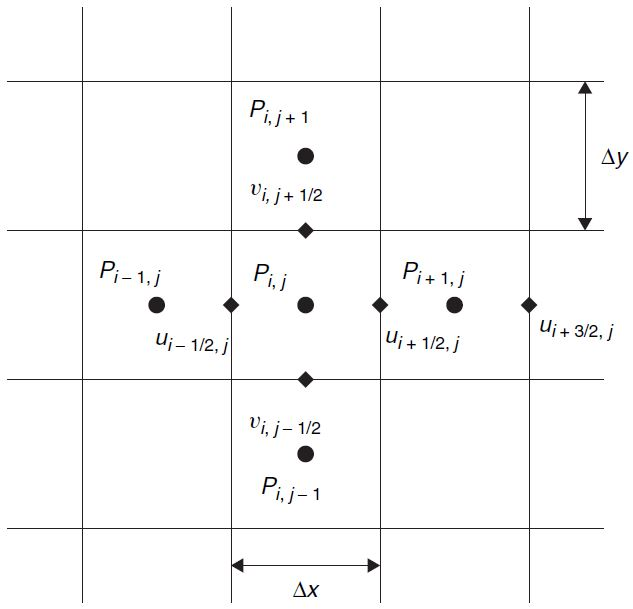
\includegraphics[height=0.395\textwidth]{grid-MAC.jpg} \label{fig:grid-MAC}}
  \subfigure[General]{\includegraphics[height=0.395\textwidth]{staggered} \label{fig:grid-staggered}}
  \subfigure[Unstructured]{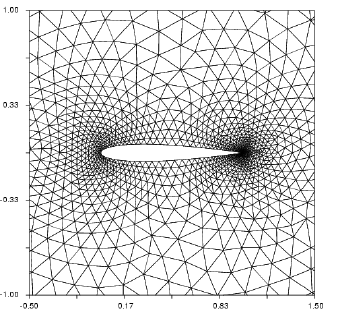
\includegraphics[height=0.265\textwidth]{grid-unstructured} \label{fig:grid-unstructured}}
\caption{\small Staggered grid.}
\end{figure}


Staggered arrangement increases complexity of a scheme and programming becomes more difficult since it requires accounting for three ($u,v,p$) or four ($u,v,w,p$) indexing systems. 
Interpolations must be used to compute nonlinear terms of momentum equations. 
Further complications arise when the grid becomes nonuniform. 
All these difficulties, however, can be relatively easily handled in computations with structured grids such as those shown in \cref{fig:grid-staggered,fig:grid-MAC}. 
The issues of handling a staggered arrangement increase significantly when unstructured (\cref{fig:grid-unstructured}) grids are used. 
When such grids started to be broadly applied in general-purpose codes recently, collocated arrangements returned to favor. 
This area of CFD is still evolving and we only mention that methods have been developed to cure the splitting problem leading to pressure oscillations. 
However, the cure is not ideal and leads to extra complexities at the implementation level.


In numerical terms, the problem \cref{eqs:NSE} can be formulated in the following way: given the solution $p^{n}$, $\boldsymbol{v}^{n}$ at the previous time layer $t^{n}$, find the next time-layer pressure $p^{n+1}$ and velocity $\boldsymbol{v}^{n+1}$ such that they together satisfy the momentum equation, the velocity is divergence-free $\nabla \cdot \boldsymbol{v}^{n+1} = 0$ and satisfies the boundary conditions.

A conspicuous feature of \cref{eqs:NSE} is that pressure $p$ is not determined by a time-evolution equation, but rather is implicitly defined by the incompressibility \cref{eqn:continuity}, which plays the role of a constraint that the velocity field $\boldsymbol{v}$ must satisfy. 
The pressure instantaneously adapts to the evolving velocity field in a way as to satisfy the constraint. 
This reflects in the fact that $p$ satisfies a Poisson equation, which can be derived by taking the divergence of \cref{eqn:momentum-intro} and combining the result with \cref{eqn:continuity}. 
From the mathematical viewpoint, this means that the incompressible flow equations have some features of an elliptic system. 
We can say that the equations belong to mixed hyperbolic (convective terms), parabolic (viscous terms), and elliptic (pressure and incompressibility) types. 
The elliptic nature of the pressure solution has a physical meaning: in an incompressible flow, the pressure field in the entire flow domain adjusts instantaneously to any, however localized, perturbation. 
This is in perfect agreement with the fact that weak perturbations, for example sound waves, propagate at infinite speed in incompressible fluids.

Given the Poisson equation for $p$, it may replace the continuity \cref{eqn:continuity} and its solution can in principle be substituted back into \cref{eqn:momentum-intro} to obtain an evolution equation for the velocity field alone. 
Alternatively, the pressure can be immediately eliminated by taking the $\mathrm{curl}$ of momentum \cref{eqn:momentum-intro}, which leads to the vorticity-stream function formulation of incompressible flow. 
Formal manipulations of this type are useful for various theoretical purposes, but the experience has shown that they are rarely advantageous for computational purposes. 
In most situations, it is preferable to simply approximate and solve \cref{eqs:NSE} directly for the so-called \textit{primitive} variables $\boldsymbol{v}$ and $p$.

If, however, one ends up solving the Poisson equation for pressure, an interesting and important question arises: "what boundary conditions should be used for the pressure field?" Such conditions are required at every point of the boundary for the Poisson problem to be well-posed. 
The conditions, however, do not naturally follow from the flow physics for the boundaries between fluid and solid walls, unless, of course, a full fluid-structure interaction problem is solved. 
Since the latter option is, in most situations, an unnecessary complication, we have to find a way to derive the pressure boundary conditions from the equations themselves.

The remainder of the present paper is organized as follows. 
	\cref{sec:vorticity-streamfunction,sec:prelude-algorithm} are dedicated to vorticity-stream function formulation and motivation for numerical scheme. 
	Formulation of the problem in terms of PDE and boundary conditions on a finite domain is performed in \cref{sec:problem-statement-dimentional,sec:nondimensionalization,sec:problem-statement-nondimensional}. 
	In \cref{sec:domain-discretization,sec:discrete-operators}, we discretize the problem. 
	Boundary conditions are discussed in \cref{sec:artificial-bc}. 
	Symmetrization of the resulting system of linear equations is performed in \cref{sec:normalization}.
	We discuss the discrete approach to the algorithm in \cref{sec:algorithm}, which is based on curl operator from \cref{subsec:curl}. 
	A summary and discussion are given in \cref{sec:summary}.
	

%\section{Discrete streamfunction method}\label{sec:discrete-streamfunction}
%%%%%%%%%%%%%%%%%%%%%%%%%%%%%%%%%%%%%%%%%%%%%%%%%%%%%%%%%%%%%%%%%%%%%%
%There are a few things to add/clarify:
%1. Non-dimensionalization.
%2. BC discussion (analytic).
%3. Symmetric BC on top to be included in all operators. 
%4. Scaling of G and D operators. 
%5. Indexation change.
%%%%%%%%%%%%%%%%%%%%%%%%%%%%%%%%%%%%%%%%%%%%%%%%%%%%%%%%%%%%%%%%%%%%%%
\todo{
\begin{itemize}
%%    \item \st{Non-dimensionalization.} \st{Shall we keep u component under value of 1? can multiply the freestream and inlet by 0.5 if needed.} Normalized to max value of 1.
%%	\item \st{Scaling of G and D operators.} \textit{$\left(C^T\right)\left(\hat{M}\right)\left(\hat{G}\right)p=\left(C^T\right)\left(\hat{M}\right)\left(\hat{M}^{-1}{G}\right)p=C^TGp=(-DC)^Tp=0$.}
%%    \item \st{Symmetric BC on top to be included in all operators.}
%%    \item \st{Indexing change for equations and figures.}
%    \item \st{Motivation.} Added some, where possible!
%    \item \st{BC discussion (analytic).} \cite{Engquist:1977,Kourta:1987,Liu:1993,Sani:1994,Persillon:1998,tsynkov:1998}.
%    \item \st{Outlet diffusion discretization is problematic. Requested PhD thesis of Jin and Persillon through UofA library. Wrote an email to their supervisor Prof. Braza and sent a message to Persillon.} Waiting for the response form UofA library since 11th Dec. 
%%    \item \st{Substitute all refs/eqrefs with smart \textbackslash cref and use one bracket for \textbackslash cite.} 
%%    \item Is it ok to use "Sys. (43)" for SLAE?
%%    \item \st{Time step $n$ is in superscript, however, domain dim's are $n\times m$, dimension index is in subscript.} Changed dimensions to $M\times N$
%%    \item Outlet idea 1. (headache division by zero) might be using uniform grid in the direction of the flow and refine grid only vertically. Will use three-point scheme into the domain, but then matrix L becomes asymmetric. 
%%	\item Outlet idea 2. Use extrapolation $\frac{\partial ^2 \boldsymbol{v}}{\partial x^2}=0$ or BC by Kourta $\frac{\partial ^2u}{\partial x^2}=0,\frac{\partial v}{\partial x	}=0$.
%    \item  \st{Found this condition $\frac{\partial \boldsymbol{v}}{\partial t}+u \frac{\partial \boldsymbol{v}}{\partial x}+v \frac{\partial \boldsymbol{v}}{\partial y}-\epsilon \frac{\partial^2 \boldsymbol{v}}{\partial y^2}=0$ by G. Fournier and F. Golanski (2008, but not many citations). They claim Prandtl BL solution for advective bc $\frac{\partial \boldsymbol{v}}{\partial t} + u\frac{\partial \boldsymbol{v}}{\partial x}=0$ is wrong, while their solution matches Prandtl BL. Looks like we can express the remaining diffusive summand in terms of pressure gradient at the boundary.} Wrote an email to author, waiting for the response. 
%    \item \st{Change computational domain to inner part only? Boundary values are to be determined by BC, not the momentum eq'n, contrary to Hall}\cite{Hall:1980}. Changed unknowns to inner part only. Values at the boundary are determined using BC. 
%    \item \st{Check algebra of diffusion and advection for $v$ component.} 
%    \item It feels like BC scheme which is consistent with inner discretization won't work, we will use Jin-Braza-Braza scheme. 
%    \item \st{Outlet BC stated early in non-dim truncated part, but discussion is much later.}
%    \item Looks like continuous analogue of $C^T$ is determined. Figured out that $C^TC=-L$ and $C^TLC=-L^2$. Some information of transpose of curl is in \href{https://www.math.mcgill.ca/gantumur/math248f19/vectorcalc.pdf}{Vector Calculus notes} on page 24 of \href{https://www.math.mcgill.ca/gantumur/math248f19/}{course by TSOGTGEREL GANTUMUR}, but the material is quite heavy.
%    \item Repeating \cref{fig:luxx-right-first} from first try of Laplacian and \cref{fig:luxx-right} after Artificial BC discussion.
%    \item Paraphrase \cite{Gamtumur:2019} in \cref{sec:algorithm} since most of it is copypaste.
%    \item Boundary conditions for \cref{eqn:biharmonic-streamfunction} are zero or non-zero.
%    \item Move discrete particular solution \cref{sec:particular-solution} to the front of algorithm \cref{sec:algorithm} and include relationship of particular solution to continuity equation with $\boldsymbol{v}=\boldsymbol{v}_p+\boldsymbol{v}_h$ in prelude to the algorithm \cref{sec:prelude-algorithm}?
%    \item change number of unknowns to include right bdry
%    \item D = -G looks ok, but pressure bc arises
%    \item curl* and curl with bc extra, curl* looks done on paper, indeed a ghost vector arises
%    \item NLBC -> L -> C'C. Here curl* looks to be not equal to C'.
%    \item TOP ABC
%    \item change top boundary condition from SYMMETRY to slip no penetration
%    \item find bc for psi in poisson of stream function. 
%    \item Change motivation in symmetrization to normalization.
	\item Dong + Chang.x
  \end{itemize}
}




\pagebreak
\section{Vorticity-stream function formulation}\label{sec:vorticity-streamfunction}
	The algorithm we will be using is a combination of classical formulation as in \cref{eqs:NSE} and vorticity transport equation \cref{eqn:transport-vorticity}.
	Consider:
	\begin{enumerate}
	\item
	Stream function $\psi(x,y,t):\boldsymbol{v}=\nabla \times \psi$ of an incompressible two-dimensional flow:
	\begin{equation}
	\label{eqn:streamfunction}
		u = \frac{\partial \psi}{\partial y},\quad v=-\frac{\partial \psi}{\partial x},
	\end{equation}
	where $\boldsymbol{v}=(u,v)$.
	
	The velocity vector at every point of space and every moment of time is tangential to the line $\psi = const$, such lines represent the streamlines of the flow. 
	\item
	
	Vorticity $\omega = \nabla \times \boldsymbol{v}$ in two-dimensional case (x-y-plane) where the only non-zero component of $\omega$ is $z$, which leads to
	\begin{equation}
	\label{eqn:vorticity}
		\omega=- \frac{\partial u}{\partial y}+\frac{\partial v}{\partial x} .
	\end{equation}
	\end{enumerate}
	
	Importantly, continuity \cref{eqn:continuity} is satisfied immediately by taking spatial derivatives of stream function \cref{eqn:streamfunction} components and adding them up. The governing \cref{eqs:NSE} can now be transformed into the following:
	\begin{enumerate}
		\item 
			Transport equation for vorticity.
			
			Applying $(\nabla \times)$ to momentum and taking into account continuity \cref{eqn:continuity} together with the fact that
			\begin{equation}
				\frac{\partial}{\partial y}\left(\frac{\partial p}{\partial x}\right) - 
				\frac{\partial}{\partial x}\left(\frac{\partial p}{\partial y}\right)=0
			\end{equation}
			will result in
			\begin{equation}
			\label{eqn:transport-vorticity}
				\boxed{
				\frac{\partial\omega}{\partial t} -\epsilon \left(\frac{\partial ^2 \omega}{\partial x^2} 
				+ \frac{\partial^2 \omega}{\partial y^2} \right)
				=-\left( u \frac{\partial\omega}{\partial x} 
				+ v\frac{\partial\omega}{\partial y}\right),
				}
			\end{equation}
			where we shifted advection terms to the right-hand side with intent to linearize them later.
		\item 
		Vorticity-Stream function equation.
		
		After substituting stream function \cref{eqn:streamfunction} into vorticity \cref{eqn:vorticity} we obtain
		\begin{equation}
			\label{eqn:vorticity-stream}
			\boxed{\nabla ^2 \psi = -\omega.}
		\end{equation}	
	\end{enumerate}
	
	The two boxed equations above form a coupled system, and the pressure field does not explicitly appear in either \cref{eqn:transport-vorticity} or \cref{eqn:vorticity-stream}. In principle, this field is not needed in the solution.
	
	The system  formed by \cref{eqn:transport-vorticity,eqn:vorticity-stream} requires boundary conditions on $\psi$ and $\omega$. 
		For the stream function imposing physically plausible conditions is not difficult. 
		One has to write the proper boundary conditions for the velocity components and use the definition of \cref{eqn:streamfunction} to represent them as  conditions for $\psi$. 
		Values for $\psi$ and its derivatives are obtained by integrating \cref{eqn:streamfunction}. In the case of vertical boundary 
		\begin{align}
			&1=u=\frac{\partial\psi}{\partial y}\implies\frac{\partial\psi}{\partial y}=1\implies\psi_1(t,y)=a_1y+a_2+\psi_2(t,x),\\
			&0=v=-\frac{\partial\psi}{\partial x}\implies\psi=\psi_1(t,y)+a_3\text{ (can be made compatible with other BCs)},		
		\end{align}
		where $a_1,a_2,a_3$ are constants. The situation is more difficult in the case of vorticity.
		There are no natural boundary conditions on $\omega$, but they can be derived from the conditions on $\psi$ by applying \cref{eqn:vorticity-stream} to the boundary. 
		The process of finding boundary conditions of $\omega$ typically results in expressions containing second derivatives, therefore, a special numerical treatment is required.





\pagebreak
\section{Prelude to the algorithm using continuous operators} \label{sec:prelude-algorithm}
We now modify momentum \cref{eqn:momentum-intro} in 2D in a similar manner as in \cref{sec:vorticity-streamfunction} with the help of differential operators. These operators can be transformed into discrete formats without much difficulty. Hence, we can apply a similar process to system of linear equations generated by \cref{eqn:momentum-intro} by multiplying it with the corresponding matrices, which is discussed in \cref{subsec:curl,sec:algorithm}. 

Define
\begin{equation}
	\operatorname{curl}
	=
	\begin{bmatrix*}[r]
	\frac{\partial}{\partial y} \\
	-\frac{\partial}{\partial x}
	\end{bmatrix*}.
\end{equation}
Hence, by stream function \cref{eqn:streamfunction} we have $\boldsymbol{v}=\operatorname{curl}\psi$. Lastly, define
\begin{equation}
	\operatorname{curl}^*
	=
	\begin{bmatrix*}[r]
	-\frac{\partial}{\partial y}&
	\frac{\partial}{\partial x}
	\end{bmatrix*}.
\end{equation}

Let us now compute $\operatorname{curl}^*$ applied to velocity vector $\boldsymbol{v}$
\begin{equation}\label{eqn:curl-adj-curl}
	\operatorname{curl}^*\boldsymbol{v}=\operatorname{curl}^*\operatorname{curl}\psi=
	\begin{bmatrix*}[r]
	-\frac{\partial}{\partial y}&
	\frac{\partial}{\partial x}
	\end{bmatrix*}
	\begin{bmatrix*}[r]
	\frac{\partial}{\partial y} \\
	-\frac{\partial}{\partial x}
	\end{bmatrix*}
	\psi
	=\left(-\frac{\partial^2}{\partial y^2} -\frac{\partial^2 }{\partial x^2}\right) \psi =-\nabla^2 \psi.
\end{equation}
By taking into account the commutativity of partial derivatives with respect to time and space we obtain
\begin{equation}\label{eqn:transient-laplacian-psi}
	\operatorname{curl}^*\left(\frac{\partial}{\partial t}\right)\operatorname{curl}\psi=-\frac{\partial}{\partial t}\left(\nabla^2 \psi \right).
\end{equation}
Applying $\operatorname{curl}^*$ to Laplacian of velocity leads to
\begin{align}\begin{split}\label{eqn:biharmonic-psi}
	\operatorname{curl}^*\nabla^2\boldsymbol{v}
	&=\operatorname{curl}^*\nabla^2\operatorname{curl}\psi\\
	&=\begin{bmatrix*}[r]
	\frac{\partial}{\partial y}&
	-\frac{\partial}{\partial x}
	\end{bmatrix*}
	\begin{bmatrix}
	\frac{\partial^2}{\partial x^2}+\frac{\partial^2}{\partial y^2} & 0\\
	0	& \frac{\partial^2}{\partial x^2}+\frac{\partial^2}{\partial y^2}
	\end{bmatrix}
	\begin{bmatrix*}[r]
	-\frac{\partial}{\partial y} \\
	\frac{\partial}{\partial x}
	\end{bmatrix*}
	\psi\\
	&=\begin{bmatrix*}[r]
	\frac{\partial}{\partial y}\left(\frac{\partial^2}{\partial x^2}+\frac{\partial^2}{\partial y^2}\right) & 0\\
	0 & -\frac{\partial}{\partial x}\left(\frac{\partial^2}{\partial x^2}+\frac{\partial^2}{\partial y^2} \right)
	\end{bmatrix*}
	\begin{bmatrix*}[r]
	-\frac{\partial}{\partial y} \\
	\frac{\partial}{\partial x}
	\end{bmatrix*}
	\psi\\
	&=-\nabla^2\left(\nabla^2\psi\right).
\end{split}\end{align}


Our goal is to obtain an equation in terms of $\psi$ by modifying \cref{eqn:momentum-intro}. 
	The procedure lies in transforming this equation into vorticity transport \cref{eqn:transport-vorticity} with the help of vorticity stream function substitution \cref{eqn:vorticity-stream} and $\operatorname{curl}$, $\operatorname{curl}^*$ operators. 
	Firstly, we put transient, gradient and viscous terms to the left-hand side, whereas non-linear terms are linearized and moved to the right. 
	Next, we substitute $\boldsymbol{v}=\operatorname{curl}\boldsymbol{\psi}$ and apply $\operatorname{curl}^*$ to rearranged momentum~\cref{eqn:momentum-intro}, which eliminates the pressure gradient ($\operatorname{curl}^*\operatorname{grad}=\begin{bmatrix*}[r]-\frac{\partial}{\partial y}&\frac{\partial}{\partial x}	\end{bmatrix*}\begin{bmatrix*}[r] \frac{\partial}{\partial x}\\ \frac{\partial}{\partial y} \end{bmatrix*}=0$). 
	For 2-dimensional case from \cref{eqn:biharmonic-psi,eqn:transient-laplacian-psi} , we get
	\begin{align}
		\operatorname{curl}^*\left( \frac{\partial \boldsymbol{v}}{\partial t} -\epsilon \nabla^2 \boldsymbol{v} \right)
			&=\operatorname{curl}^*\left( \boldsymbol{v}\cdot\nabla\boldsymbol{v}\right)\\
		\operatorname{curl}^*\left( \frac{\partial }{\partial t}\operatorname{curl}\psi -\epsilon \nabla^2 \operatorname{curl}\psi \right)
			&=\operatorname{curl}^*\left( \boldsymbol{v}\cdot\nabla\boldsymbol{v}\right)\\
		\left(\frac{\partial}{\partial t} -\epsilon \nabla^2\right)\left(-\nabla^2\psi\right)
			&=\operatorname{curl}^*\left( \boldsymbol{v}\cdot\nabla\boldsymbol{v}\right)\label{eqn:biharmonic-heat-eqn}
	\end{align}
	
	Solving \cref{eqn:biharmonic-heat-eqn} for $\nabla^2\psi$ is equivalent to obtaining a solution for Poisson \cref{eqn:vorticity-stream}. However, we can go through \cref{eqn:biharmonic-heat-eqn} and solve it in one step by obtaining $\psi$ from biharmonic equation
	\begin{equation}
	\label{eqn:biharmonic-streamfunction}
		\boxed{
		-\frac{\partial\nabla ^2 \psi}{\partial t} 
		+\epsilon\nabla ^4 \psi=\operatorname{curl}^*\left( \boldsymbol{v}\cdot\nabla\boldsymbol{v}\right),
		}
	\end{equation}
where the right-hand side contains boundary conditions (in numerical sense) and non-linear advective terms, which were initially stated in terms of $\boldsymbol{v},p$ and transformed through premultiplication by $\operatorname{curl}^T$. 





\subsection{Vector fields that vanish at the boundary}
This subsection contains side notes for \cref{sec:prelude-algorithm}, here we discuss some properties of differential operators in vector calculus. Consider continuous operators $\operatorname{div}$, $\operatorname{curl}$ and $\operatorname{grad}$ on bounded domain $\Omega$ with boundary $\partial \Omega$. Let all vector $\boldsymbol{X},\boldsymbol{Y}$ and scalar $\phi,\psi$ fields vanish at $\partial \Omega$. Denote by $SF$ the set of all scalar fields in $\Omega$, and by $VF$ the set of all vector fields in $\Omega$. In this subsection we need to have inner products in inner product space \cite{Gamtumur:2019}. Define scalar and vector inner products as
\begin{equation}
	\langle\phi, \psi\rangle=\int_{\Omega} \phi \psi\ dV,\quad
	\langle \boldsymbol{X}, \boldsymbol{Y}\rangle=\int_{\Omega} \boldsymbol{X} \cdot \boldsymbol{Y}\ dV.
\end{equation}
Then define the transpose of grad as an operator $\operatorname{grad}^T: V F \rightarrow S F$ such that
\begin{equation}
	\langle  \operatorname{grad} \phi,\boldsymbol{X}\rangle=\left\langle\phi, \operatorname{grad}^T \boldsymbol{X}\right\rangle,
\end{equation}
for all vector fields $\boldsymbol{X}$ and scalar fields $\phi$ vanishing at the boundary $\partial \Omega$. To identify this operator, integrate the identity
\begin{equation}
	\nabla \cdot(\phi \boldsymbol{X})= \nabla \phi\cdot \boldsymbol{X}+ \phi \nabla \cdot \boldsymbol{X},
\end{equation}
and apply the divergence theorem, to get
\begin{equation}\label{eqn:div-grad}
	\int_{\partial \Omega} \phi \boldsymbol{X} \cdot \boldsymbol{n}\ dS=\int_{\Omega} \nabla \cdot(\phi \boldsymbol{X})\ dV=\int_{\Omega} \nabla \phi\cdot \boldsymbol{X}\ dV +\int_{\Omega} \phi \nabla \cdot \boldsymbol{X}\ dV.
\end{equation}
Since $\phi=0$ on $\partial \Omega$, left side of \cref{eqn:div-grad} vanishes. Hence, we infer
\begin{equation}\label{eqn:inner-grad-div}
	0=\langle \nabla \phi,\boldsymbol{X}\rangle+\langle\phi, \nabla \cdot \boldsymbol{X}\rangle,
\end{equation}
implying that the transpose of the gradient is the negative divergence, and the transpose of the divergence is the negative gradient:
\begin{equation}\label{eqn:curl-grad}
	\operatorname{grad}^T=- \text { div }, \quad \text { div }^T=-\operatorname{grad} .
\end{equation}

We now move to the 3-dimensional case, consider the following identity
\begin{equation}
\nabla \cdot(\boldsymbol{X} \times \boldsymbol{Y})=(\nabla \times \boldsymbol{X}) \cdot \boldsymbol{Y}-\boldsymbol{X} \cdot(\nabla \times \boldsymbol{Y}).
\end{equation}
Navier-Stokes \cref{eqs:NSE} are defined in the whole domain from $-\infty$ to $+\infty$ in each axis. 
	In our problem operators $\operatorname{curl},\operatorname{grad},\operatorname{div}$ are local. 
	Therefore, we are allowed to let velocity vector fields vanish at the boundaries $\pm\infty$.
	Since we consider only those vector fields that go to zero at $\partial \Omega$, the divergence theorem yields
\begin{multline}
	0
	=	\int_{\partial \Omega}(\boldsymbol{X} \times \boldsymbol{Y}) \cdot \boldsymbol{n}\ dS
	=\int_{\Omega} \nabla \cdot(\boldsymbol{X} \times \boldsymbol{Y})\ dV=\\
	=\int_{\Omega} \left(\nabla \times \boldsymbol{X}\right)\cdot \boldsymbol{Y}\ dV
		-\int_{\Omega} \boldsymbol{X} \cdot \left(\nabla \times \boldsymbol{Y}\right)\ dV
	=\langle \operatorname{curl}\boldsymbol{X},\boldsymbol{Y}\rangle-\langle \boldsymbol{X},\operatorname{curl}^T\boldsymbol{Y}\rangle ,
\end{multline}
which identifies the curl as the transpose of itself in 3D:
\begin{equation}\label{eqn:curl-curl-orth}
\operatorname{curl}^T=\operatorname{curl.}	
\end{equation}


\pagebreak
\section{Problem statement}\label{sec:problem-statement-dimentional}
Let the velocity vector $\boldsymbol{v}(t,x,y)=(u(t,x,y),v(t,x,y))$ and pressure $p(t,x,y)$ be the solutions to ~\cref{eqs:NSE} on a semi-infinite domain together with boundary conditions:
\begin{subequations}
\label[pluralequation]{eqs:NSE-dsm-bl-dimensional}
\begin{align}
\label{eqn:momentum-dimensional}
\text{Momentum: }	&\frac{\partial \boldsymbol{v}}{\partial t} + \boldsymbol{v} \cdot \nabla \boldsymbol{v} = -\frac{1}{\rho}\nabla p + {\frac{\mu}{\rho}} \nabla \cdot \nabla \boldsymbol{v},\\
&\rho\text{ - density}, \mu\text{ - dynamic viscosity.}\notag\\
\label{eqn:continuity-dsm-bl}
\text{Continuity: }	& \nabla \cdot \boldsymbol{v} = 0, \\ 
					&0\leq x < \infty, 0\leq y <\infty, t\geq0.\notag\\
\label{eqn:NSE-dsm-bl-bc-freestream}
\text{Inlet and Freestream BC: } 	& \boldsymbol{v}(t,0,y)=\boldsymbol{v}(t,x,\infty)=\left(U_0 + A\cos\left( kx -\omega t + \phi_0 \right),0\right),\\
									& \{|A|<U_0,k,\omega, \phi_0\}\subset \mathbb{R}.\notag\\
\label[bc]{eqn:NSE-dsm-bl-bc-noslip}
\text{No-slip BC: } & \boldsymbol{v}(t,x,0)=(0,0). \\
%\label{eqn:NSE-dsm-bl-bc-outlet}
%\text{Outlet BC: } 	& \frac{\partial u}{\partial t}+u\frac{\partial u}{\partial x}=0\lor\left(\frac{\partial u}{\partial t}+u\frac{\partial u}{\partial x}=\epsilon \frac{\partial ^2 u}{\partial y^2}\right), \\ 
%					& v=\boldsymbol{h}(t,y)-\text{linear extrapolation},\notag\\
%					& (x=\infty),\notag\\
\text{Initial condition: } &\boldsymbol{v}(0,x,y)=(0,0) \text{ or Blasius profile.}
\end{align}
\end{subequations}



%\subsubsection{Top BC}\label{subsubsec:top-bc}

\section{Nondimensionalization}\label{sec:nondimensionalization}
In numerical computations, it is advantageous to maintain variables of comparable magnitude. This ensures that operations such as the multiplication of a large dimensional pressure variable with a small velocity are not performed. 

We will truncate the domain and normalize all equations by width $L$ and stream velocity $U_0$. After introducing the following dimensionless variables (marked with prime ${ }^{\prime}$ ):
\begin{equation*}
	x\to Lx^{\prime},  \quad 
	\boldsymbol{v}\to U_0\boldsymbol{v}^{\prime}, \quad 
	\nabla\to \frac{1}{L}\nabla^{\prime}, \quad 
%	\Delta \to \frac{1}{L^2} \Delta^{\prime},  \quad 
	p\to p^{\prime} \rho U_0^2, \quad 
	t\to \frac{L}{U_0}t^{\prime},
\end{equation*}
we obtain
\begin{equation*}
	\frac{U_0}{\frac{L}{U_0}} \frac{\partial \boldsymbol{v}^{\prime}}{\partial t^{\prime}}+U_0\boldsymbol{v}\cdot\left(\frac{1}{L} \nabla^{\prime}\right) U_0\boldsymbol{v}=-\frac{1}{\rho}\left(\frac{1}{L} \nabla^{\prime}\right){p^{\prime}\rho U^2_0}+\frac{\mu}{\rho} \left(\frac{1}{L} \nabla^{\prime}\right) \cdot\left(\frac{1}{L} \nabla^{\prime}\right) U_0\boldsymbol{v}^{\prime}.
\end{equation*}
After multiplying both sides of the above identity by $\frac{L}{U_0^2}$ and introducing well-known Reynolds number 
\begin{equation*}
\operatorname{Re}=\frac{\rho L U_0}{\mu}
\end{equation*}
we obtain the non-dimensional momentum equation
\begin{equation*}
	\frac{\partial \boldsymbol{v}}{\partial t} + \boldsymbol{v} \cdot \nabla \boldsymbol{v} = -\nabla p + \frac{1}{\operatorname{Re}} \nabla \cdot \nabla \boldsymbol{v},
\end{equation*}
where prime superscript $\prime$ is suppressed for the dimensionless variables. 

The continuity equation is nondimensionalized in a similar manner:
\begin{equation*}
	\left(\frac{1}{L} \nabla^{\prime}\right) \cdot U_0\boldsymbol{v}^{\prime}=0\iff\nabla^{\prime} \cdot\boldsymbol{v}^{\prime}=0\implies\nabla \cdot\boldsymbol{v}=0,
\end{equation*}
where we drop prime superscripts in the last identity as well.

\pagebreak
\section{Problem statement on truncated domain}\label{sec:problem-statement-nondimensional}
The initial \cref{eqs:NSE-dsm-bl-dimensional} from \cref{sec:problem-statement-dimentional} on semi-infinite domain now become a system of partial differential equations on a unit square domain 
\begin{subequations}
\label[pluralequation]{eqs:NSE-dsm-bl}
\begin{align}
\label{eqn:momentum}
\text{Momentum: }	&\frac{\partial \boldsymbol{v}}{\partial t} + \boldsymbol{v} \cdot \nabla \boldsymbol{v} = -\nabla p + \epsilon \nabla \cdot \nabla \boldsymbol{v}, \\ 
					&\epsilon = \frac{1}{\operatorname{Re}},0\leq x \leq 1, 0\leq y \leq 1, t\geq0.\notag\\
\label{eqn:continuity-dsm-bl}
\text{Continuity: }	& \nabla \cdot \boldsymbol{v} = 0, \\ 
					&0\leq x \leq 1, 0\leq y \leq 1, t\geq0. \notag\\
\label[bc]{eqn:NSE-dsm-bl-bc-freestream}
\text{Inlet: } 	& \boldsymbol{v}(t,0,y)=\boldsymbol{v}(t,x,1)=\left(1 + A\cos\left( kx -\omega t + \phi_0 \right),0\right),\\
									& \{A\leq 1,k,\omega, \phi_0\}\subset \mathbb{R}.\notag\\
\label[bc]{eqn:NSE-dsm-bl-bc-noslip}
\text{No-slip wall BC: } & \boldsymbol{v}(t,x,0)=(0,0). \\
\label[bc]{eqn:NSE-dsm-bl-bc-open}
\text{Outlet and freestream BC: } 	&\text{Artificial boundary conditions.} \notag\\
					&\text{Details are discussed in \cref{sec:artificial-bc}.}\notag\\
\text{Initial condition: } &\boldsymbol{v}(0,x,y)=(0,0)\text{ or Blasius profile}.
\end{align}
\end{subequations}

\section{Domain discretization}\label{sec:domain-discretization}
Following the nondimensionalization of the governing equations, we now turn our attention to the process of domain discretization. 
This crucial step involves dividing the computational domain into discrete elements, allowing us to compute variables and their derivatives on a finite set of points called the grid. 
Consider discretizing the area into $M$ intervals horizontally and $N$ intervals vertically forming a mesh of rectangular cells. 
To enhance the code it is recommended to organize the data using vectors instead of matrices in order to improve memory access time; a single index $i$ works faster than double $i,j$ in most programming languages. 
In this section, however, for the sake of simplicity, we use two indices $i,j$ (column and row as in Harlow and Welch~\cite{Harlow:1965}) to represent coordinates on the grid.

\begin{figure}[H] % here, bottom, top
  \centering{
  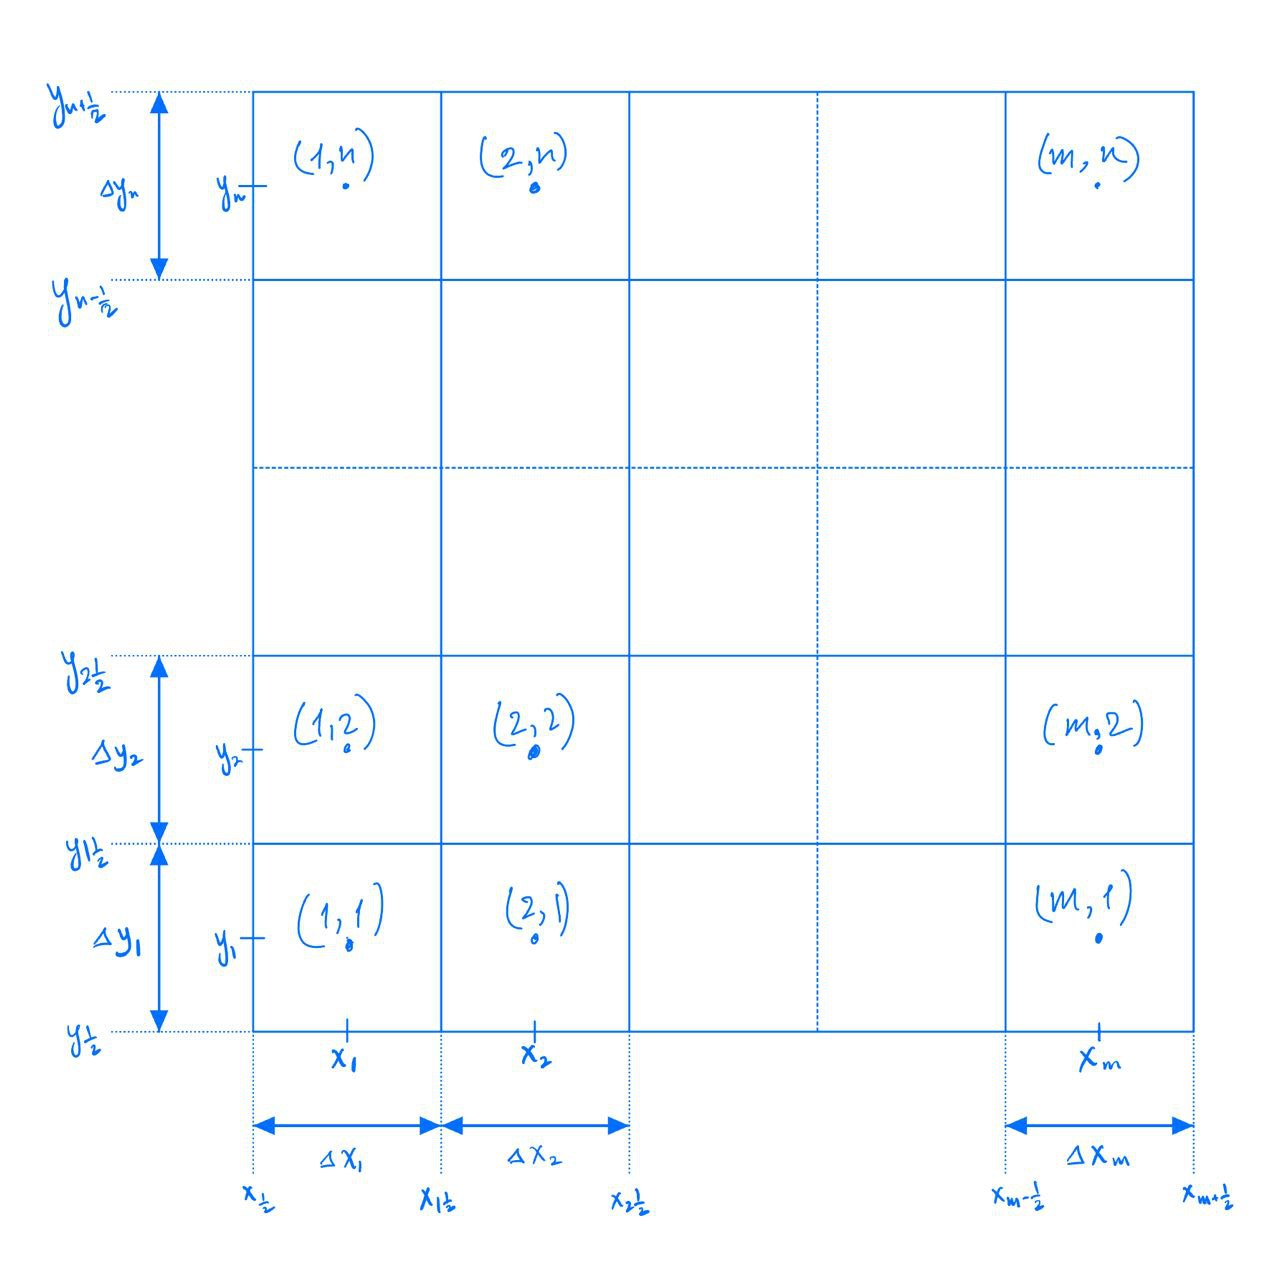
\includegraphics[width=0.40\paperwidth]{grid-bl}
  }
  \caption{Domain discretization (here $m=M, n=N$)}\label{bl-domain-discretization}
\end{figure}

To eliminate the necessity of solving an additional equation for pressure we will be using a staggered grid arrangement. 
	Details are discussed in \cref{subsec:divergence,subsec:gradient,subsec:curl}. 
	Moreover, the pressure gradients can be evaluated directly using central differences on such grids. 
	This calculation on staggered grids does not require any interpolation, furthermore, it is computationally cheaper and simpler to implement. 

The $u$ velocity components are stored at the centres of vertically oriented faces, while the values of $v$ are stored at the centres of horizontal ones. 
	The number of momentum equations is $(M+1)N$ for $v$ and $M(N+1)$ for $u$. 
	These arrays for $u$ and $v$ are then concatenated into a single vector $\boldsymbol{v}$ of size $M(N+1)+(M+1)N$.

Increasing the accuracy closer to the wall and the inlet does look advantageous, hence, we will refine the grid using the standard ratio rule $\Delta x_{i+1}=k_x\Delta x_i,\Delta y_{j+1}=k_y\Delta y_j$ with constants $k_x,k_y$ of values close to $1$. 
	


%%%%%%%%%%%%%%%%%%%%%%%%%%%%%%%%%%%%%%%%%%%%%%%%%%%%%%%%
\pagebreak
\section{Discrete operators}\label{sec:discrete-operators}

This subsection focuses on the specific operators used in the discretization of \cref{eqs:NSE-dsm-bl}, providing the mathematical tools necessary to transform these continuous equations into a form that can be solved numerically.

Denote discrete spatial operators as:
\begin{enumerate}
	\item[$\hat{L}$]:  Laplacian.
	\item[$\hat{G}$]: Gradient.
	\item[$\hat{D}$]: Divergence.
	\item[$\mathbf{\hat{H}}$]: Non-linear advective terms.
\end{enumerate}
Then original system of \cref{eqs:NSE-dsm-bl} can be approximated using such operators as
\begin{equation}\label[system]{eqn:nse-matrix}
            \begin{bmatrix}
                  \mathbf{I} && 0 \\ 
                  0 && 0
            \end{bmatrix}
            \frac{\partial }{\partial t} 
            \begin{pmatrix}
                  \boldsymbol{v} \\ 
                  p
            \end{pmatrix}
            =
            \begin{bmatrix}
                  \hat{L} && - \hat{G} \\ 
                  -\hat{D} && 0
            \end{bmatrix}
            \begin{bmatrix}
                  \boldsymbol{v} \\
                  p
            \end{bmatrix}
            +
            \begin{pmatrix}
                  -\mathbf{\hat{H}}(\boldsymbol{v})\\
                  0
            \end{pmatrix} + \text{bc}_{\boldsymbol{v},p},
        \end{equation}
where boundary conditions are in terms of pressure and velocity. In the following subsections, each of the discrete operators is described individually. 

%%%%%%%%%%%%%%%%%%%%%%%%%%%%%%%%%%%%%%%%%%%%%%%%%%%%%%%%%%%
%\subsubsection{Transient terms}\label{subsec:transient}
Attack \cref{eqn:nse-matrix} with the following schemes as in Colonius~\cite{Colonius:2008} (superscript denotes the time step):
\begin{enumerate}
	\item[\textbf{Viscous}] - Implicit trapezoidal - Crank Nicholson scheme (second-order method in time).  
%	\begin{equation}\label{eqn:crank-nicholson}
%		\frac{\boldsymbol{v}^{n+1}-\boldsymbol{v}^n}{\Delta t}=\frac{1}{2}\left[F^{n+1}+F^n\right],
%	\end{equation}
	\begin{equation}\label{eqn:viscous-crank-nicholson}
  		\hat{L}\boldsymbol{v}=\frac{1}{2}\left(\hat{L}\boldsymbol{v}^{n+1}+\hat{L}\boldsymbol{v}^n\right).
	\end{equation}

	\item[\textbf{Nonlinear}] - Explicit Adams-Bashforth (second-order method in time).
%	\begin{equation}\label{eqn:adams-bashforth}
%		\frac{\boldsymbol{v}^{n+1}-\boldsymbol{v}^{n}}{\Delta t} = \frac{3}{2}F^{n} - \frac{1}{2}F^{n-1}.
%	\end{equation}
	\begin{equation}\label{eqn:nonlinear-adams-bashforth}
		\mathbf{\hat{H}}(\boldsymbol{v}) = \frac{3}{2}\mathbf{\hat{H}}(\boldsymbol{v}^{n}) - \frac{1}{2}\mathbf{\hat{H}}(\boldsymbol{v})^{n-1}.
	\end{equation}

	\item[\textbf{Pressure}] - Implicit Euler, though the pressure variable will be later eliminated in the algorithm (first-order method in time). 
%	\begin{equation}\label{eqn:implicit-euler} 
%		\frac{\boldsymbol{v}^{n+1}-\boldsymbol{v}^{n}}{\Delta t} = F^{n+1}.
%	\end{equation}
	\begin{equation}\label{eqn:pressure-implicit-euler} 
		\hat{G}p = \hat{G}p^{n+1}.
	\end{equation}
\end{enumerate}

The schemes above result in the following time-discretized system:
\begin{equation}\label[system]{eqn:NSE-dsm-bl-system-schemes}
	\begin{bmatrix}
		\frac{1}{\Delta t}\mathbf{I}-\frac{1}{2}\hat{L} & \hat{G} \\
		\hat{D} & 0
	\end{bmatrix}
	\begin{pmatrix}
		\boldsymbol{v}^{n+1} \\ 
		p^{n+1}
	\end{pmatrix}
	=
	\begin{pmatrix}
		\left[\frac{1}{\Delta t}\mathbf{I}-\frac{1}{2}\hat{L}\right] \boldsymbol{v}^n - \left[\frac{3}{2}\hat{\mathbf{H}}(\boldsymbol{v}^n) - \frac{1}{2}\hat{\mathbf{H}}(\boldsymbol{v}^{n-1})\right]\\
		0
	\end{pmatrix}
	+
	\begin{pmatrix}
		\hat{bc}_1\\
		\hat{bc}_2
	\end{pmatrix}.
\end{equation}
%and \cref{eqn:Jin-Braza-bc} 
%\begin{equation}\label[bc]{eqn:Jin-Braza-bc-transient-consistent}
%\begin{gathered}
%\frac{\boldsymbol{v}^{n+1}-\boldsymbol{v}^n}{\Delta t}+\left[\frac{3}{2}{u^n}\left(\frac{\partial \boldsymbol{v}}{\partial x}\right)^{n}-\frac{1}{2}{u^{n-1}}\left(\frac{\partial \boldsymbol{v}}{\partial x}\right)^{n-1}\right] \\
%=\epsilon\left[\left(\frac{\partial^2 \boldsymbol{v}}{\partial y^2}\right)^{n+1}+\left(\frac{\partial^2 \boldsymbol{v}}{\partial y^2}\right)^{n}\right],
%\end{gathered}
%\end{equation}
%however, the results produced with such \cref{eqn:Jin-Braza-bc-transient-consistent} schemes are yet to be known and should be compared with \cref{eqn:Jin-Braza-bc-transient} from the corresponding paper of Jin-Braza\cite{Jin:1993}, which was said to be 
%\begin{equation}\label[bc]{eqn:Jin-Braza-bc-transient}
%\begin{gathered}
%\frac{\boldsymbol{v}^{n+1}-\boldsymbol{v}^n}{\Delta t}+\frac{u^n}{2}\left[\left(\frac{\partial \boldsymbol{v}}{\partial x}\right)^{n+1}+\left(\frac{\partial \boldsymbol{v}}{\partial x}\right)^n\right] \\
%=\epsilon\left(\frac{\partial^2 \boldsymbol{v}}{\partial y^2}\right)^n.
%\end{gathered}
%\end{equation}
We will use artificial boundary conditions from Dong~\cite{Dong:2014} to generate boundary contributions of outlet and freestream to $\hat{bc_1}$. Their condition was shown to be stable and produced solid results. Details are discussed in \cref{sec:artificial-bc}.

After applying the discrete operators (listed in the following \cref{subsec:advection,sec:laplacian,subsec:divergence,subsec:gradient}) and making a substitution for explicit terms, we rewrite \cref{eqn:NSE-dsm-bl-system-schemes}  as
\begin{equation}\label[system]{eqn:NSE-dsm-bl-system-nonint}
	\boxed{\begin{bmatrix}
		\hat{A} & \hat{G} \\
		\hat{D} & 0
	\end{bmatrix}
	\begin{pmatrix}
		\boldsymbol{v}^{n+1} \\ 
		p^{n+1}
	\end{pmatrix}
	=
	\begin{pmatrix}
		\hat{r}^n \\
		0
	\end{pmatrix}
	+
	\begin{pmatrix}
		\hat{bc}_1\\
		\hat{bc}_2
	\end{pmatrix},}
\end{equation}
where $\hat{r}^n=\left[\frac{1}{\Delta t}\mathbf{I}-\frac{1}{2}\hat{L}\right] \boldsymbol{v}^n - \left[\frac{3}{2}\hat{\mathbf{H}}(\boldsymbol{v}^n) - \frac{1}{2}\hat{\mathbf{H}}(\boldsymbol{v}^{n-1})\right]$ includes viscous, non-linear and gradient terms from time steps $n,n-1$ and $\hat{bc}_i$ are explicit boundary values in terms of velocity and pressure.


%%%%%%%%%%%%%%%%%%%%%%%%%%%%%%%%%%%%%%%%%%%%%%%%%%%%%%%%%%%


%%%%%%%%%%%%%%%%%%%%%%%%%%%%%%%%%%%%%%%%%%%%%%%%
\subsection{Advection}\label{subsec:advection}

Since Explicit Adams-Bashforth~\cref{eqn:nonlinear-adams-bashforth} uses information from time steps $n$ and $n-1$, while we solve the system of equations for time step $n+1$, there is no need for upwind or even more complicated schemes. 
For spatial discretization we will try to stick to the central schemes. 
Such approximations are more stable and less dependent on the flow direction. 
It is convenient to write these schemes for a conservative form of the advection. 
Moreover, such an approach also keeps the error low, since there is no product of velocity with acceleration. 
Hence, let us rewrite advective derivatives in conservative form. 
\begin{align}\label{eqn:advection-conservative}
	u\frac{\partial u}{\partial x}+v \frac{\partial u}{\partial y}
	&=u\frac{\partial u}{\partial x}+0+v \frac{\partial u}{\partial y}\nonumber\\
	&= u\frac{\partial u}{\partial x}+ u\left(\frac{\partial u}{\partial x} +\frac{\partial v}{\partial y}\right ) +v \frac{\partial u}{\partial y}\nonumber\\
	&=\left(u\frac{\partial u}{\partial x}+ u\frac{\partial u}{\partial x}\right ) +\left(u\frac{\partial v}{\partial y} +v \frac{\partial u}{\partial y}\right )\nonumber\\
	&=\frac{\partial uu}{\partial x}+ \frac{\partial uv}{\partial y}.
\end{align}
Our goal now is to approximate advection components for each momentum equation. Below we will describe the discretization schemes for \cref{eqn:advection-conservative}. 

\subsubsection{Inner part}\label{subsubsec:advection-inner}
\begin{figure}[H] % here, bottom, top
  \centering{
  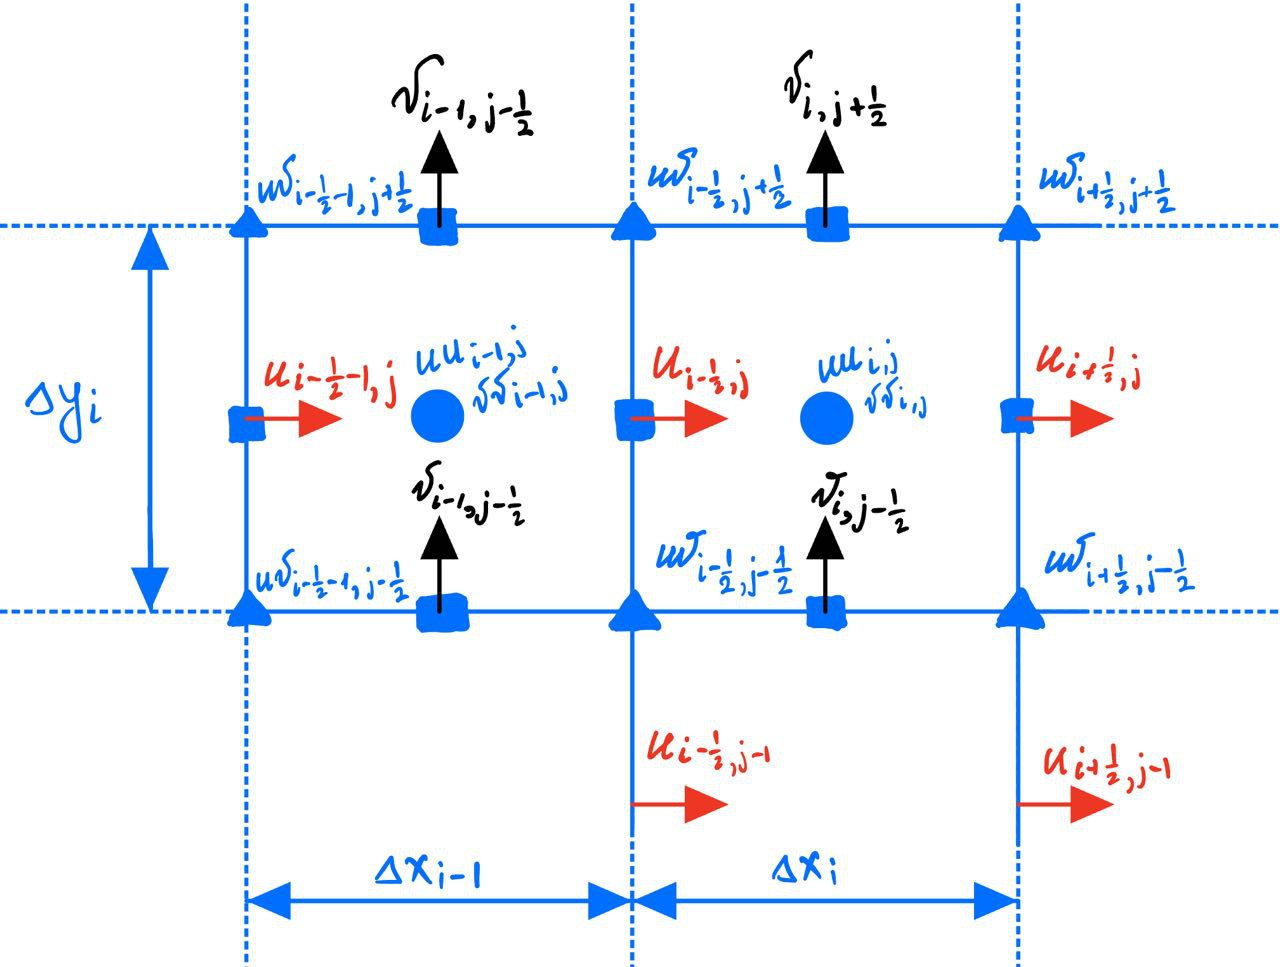
\includegraphics[width=0.65\paperwidth]{ADV}
  }
  \caption{Advection discretization.}\label{fig:ADV}
\end{figure}
The advective component from $x$-momentum was expressed in conservative form by \cref{eqn:advection-conservative}. It is discretized using the standard central differencing schemes~\cite{Colonius:2008} as
\begin{align}\label{eqn:adv-inner}
	\left (u\frac{\partial u}{\partial x}+v \frac{\partial u}{\partial y}\right)_{i-\frac{1}{2},j}&=\frac{(uu)_{i
	,j}-(uu)_{i- 1,j}}{\frac{\Delta x_i+\Delta x_{i-1}}{2}}+\frac{(uv)_{i-\frac{1}{2},j+\frac{1}{2}}-(uv)_{i-\frac{1}{2},j-\frac{1}{2}}}{\Delta y_i},
\end{align}
which is evaluated at the same points as $u_{i-\frac{1}{2},j}$ (squares in \cref{fig:ADV}). It is required to compute $uv$ at the nodes and $uu$ at the cell centres, which are triangles and circles respectively in \cref{fig:ADV}. Using linear interpolation~\cite{Colonius:2008} of velocity values leads to:
\begin{align*}
  (uu)_{i,j}&=\left(\frac{u_{i+\frac{1}{2},j}+u_{i-\frac{1}{2},j}}{2}\right)^2,\\
  (uv)_{i-\frac{1}{2},j-\frac{1}{2}}&=\left(u_{i-\frac{1}{2},j-1} + \frac{\Delta y_{j-1}}{2}\frac{u_{i-\frac{1}{2},j}-u_{i-\frac{1}{2},j-1}}{\frac{\Delta y_{j-1} +\Delta y_j}{2}} \right) \left( v_{i-1,j-\frac{1}{2}} + \frac{\Delta x_{i-1}}{2}\frac{v_{i,j-\frac{1}{2}}-v_{i-1,j-\frac{1}{2}}}{\frac{\Delta x_{i-1} +\Delta x_i}{2}}\right)\\
  &=\left(\frac{u_{i-\frac{1}{2},j}\Delta y_{j-1} +u_{i-\frac{1}{2},j-1}\Delta y_j}{\Delta y_{j-1}+\Delta y_{j}}\right )\left ( \frac{v_{i,j-1\frac{1}{2}}\Delta x_{i-1} +v_{i-1,j-\frac{1}{2}}\Delta x_i}{\Delta x_{i-1}+\Delta x_{i}}\right).
\end{align*}


\subsubsection{Left boundary}\label{subsubsec:advection-left}
\begin{figure}[H] % here, bottom, top
  \centering{
  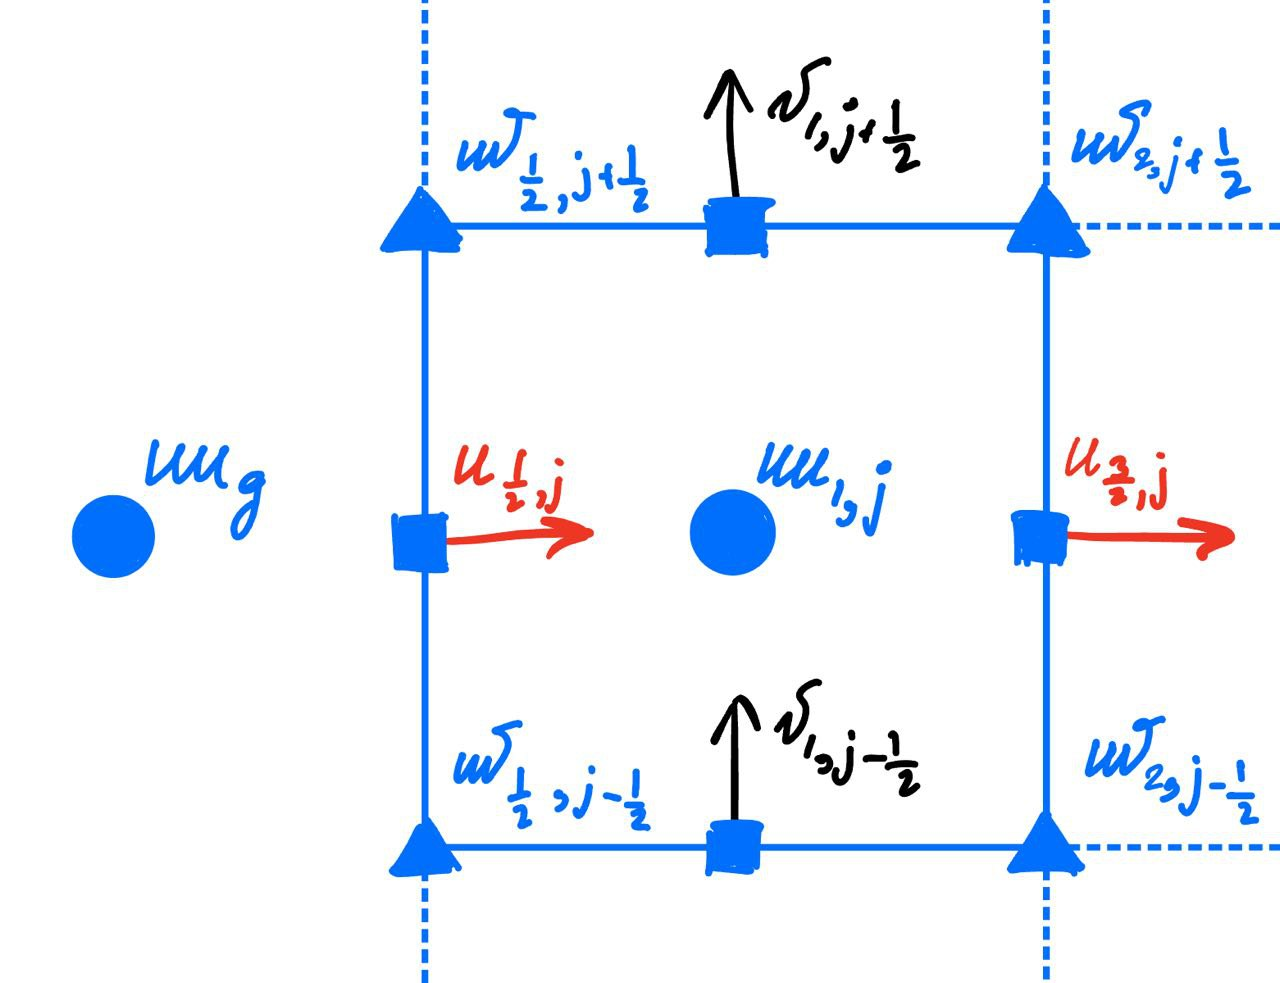
\includegraphics[width=0.30\paperwidth]{ADV-left}
  }
  \caption{Left boundary advection.}\label{fig:ADV-left}
\end{figure}
The exact value of the $uu_g$ element, which is located outside the boundary (\cref{fig:ADV-left}), is known from the inlet boundary conditions, whereas $uv_{\frac{1}{2},j}$ is zero for all $j$ due to $v_{bc}=0$ at the inlet. 

\subsubsection{Bottom boundary}\label{subsubsec:advection-bottom}
\begin{figure}[H] % here, bottom, top
  \centering{
  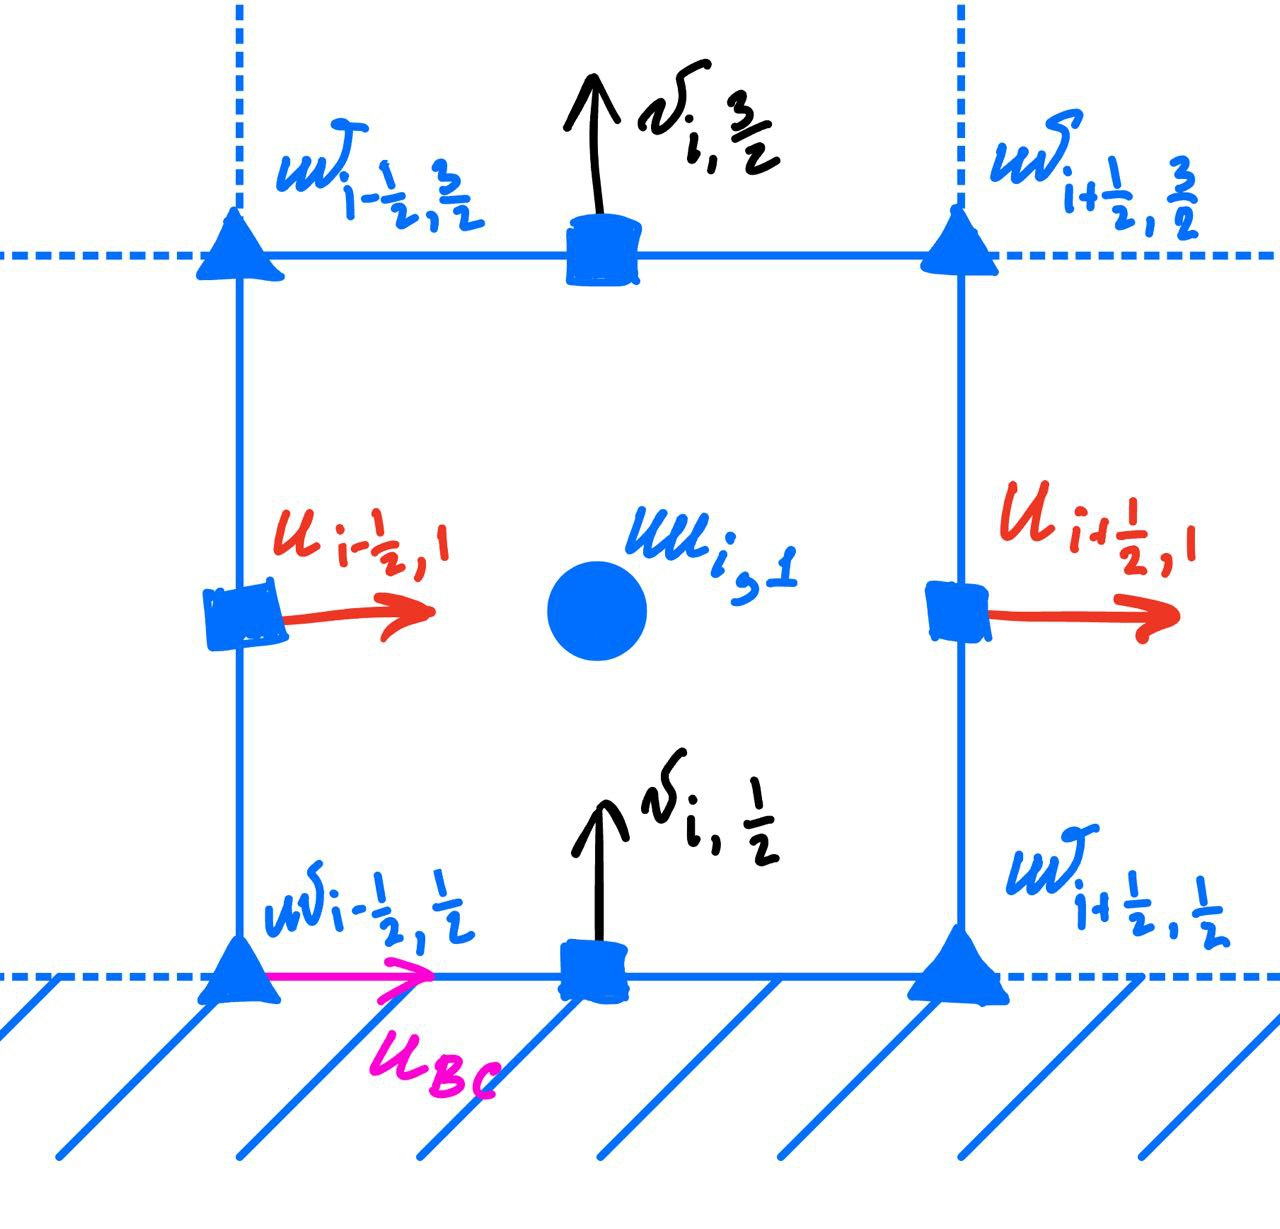
\includegraphics[width=0.30\paperwidth]{ADV-bottom}
  }
  \caption{Bottom boundary advection}\label{fig:ADV-bottom}
\end{figure}
Computation of the advective terms just above the bottom boundary is verbatim to the inner part, with the only exception being $uv_{i-\frac{1}{2},\frac{1}{2}}=0$ at the boundary due to the $u_{bc}=0$ condition on the plate (purple on \cref{fig:ADV-bottom}).

The advective terms in the $y$-momentum equation are computed in a similar manner. After the derivatives are evaluated, they are moved to the right-hand side as in \cref{eqn:NSE-dsm-bl-system-schemes} and treated explicitly. 

\subsubsection{Right and top boundaries}\label{subsubsec:advection-right}

We will use standard linear extrapolation to compute necessary velocity products $uu$, $vv$ and $uv$ that lie outside and at the boundary. Computational process for both of these are exactly the same:
\begin{equation}
	uu_{M+1,j}=uu_{M-1,j}+\left( \frac{\Delta x_{M-1}}{2}+\Delta x_M + \frac{\Delta x_{M+1}}{2} \right)\frac{uu_{M,j}-uu_{M-1,j}}{\frac{\Delta x_M+\Delta x_{M-1}}{2}},
\end{equation}
\begin{equation}
	vv_{M+1,j}=vv_{M-1,j}+\left( \frac{\Delta x_{M-1}}{2}+\Delta x_M + \frac{\Delta x_{M+1}}{2} \right)\frac{vv_{M,j}-vv_{M-1,j}}{\frac{\Delta x_M+\Delta x_{M-1}}{2}}.
\end{equation}
Components $uv$ located at the nodes are approximated as
\begin{equation}
	uv_{M+\frac{1}{2},j-\frac{1}{2}}=uv_{M-\frac{3}{2},j}+\left( {\Delta x_{M-1}}+\Delta x_M  \right)\frac{uv_{M-\frac{1}{2},j-\frac{1}{2}}-uv_{M-\frac{3}{2},j-\frac{1}{2}}}{\Delta x_{M-1}}.
\end{equation}


At the top boundary $\Delta x$ will change to $\Delta y$ and extrapolation will be performed for vertical indices rather than horizontal. 

\begin{figure}[H] % here, bottom, top
  \centering{
  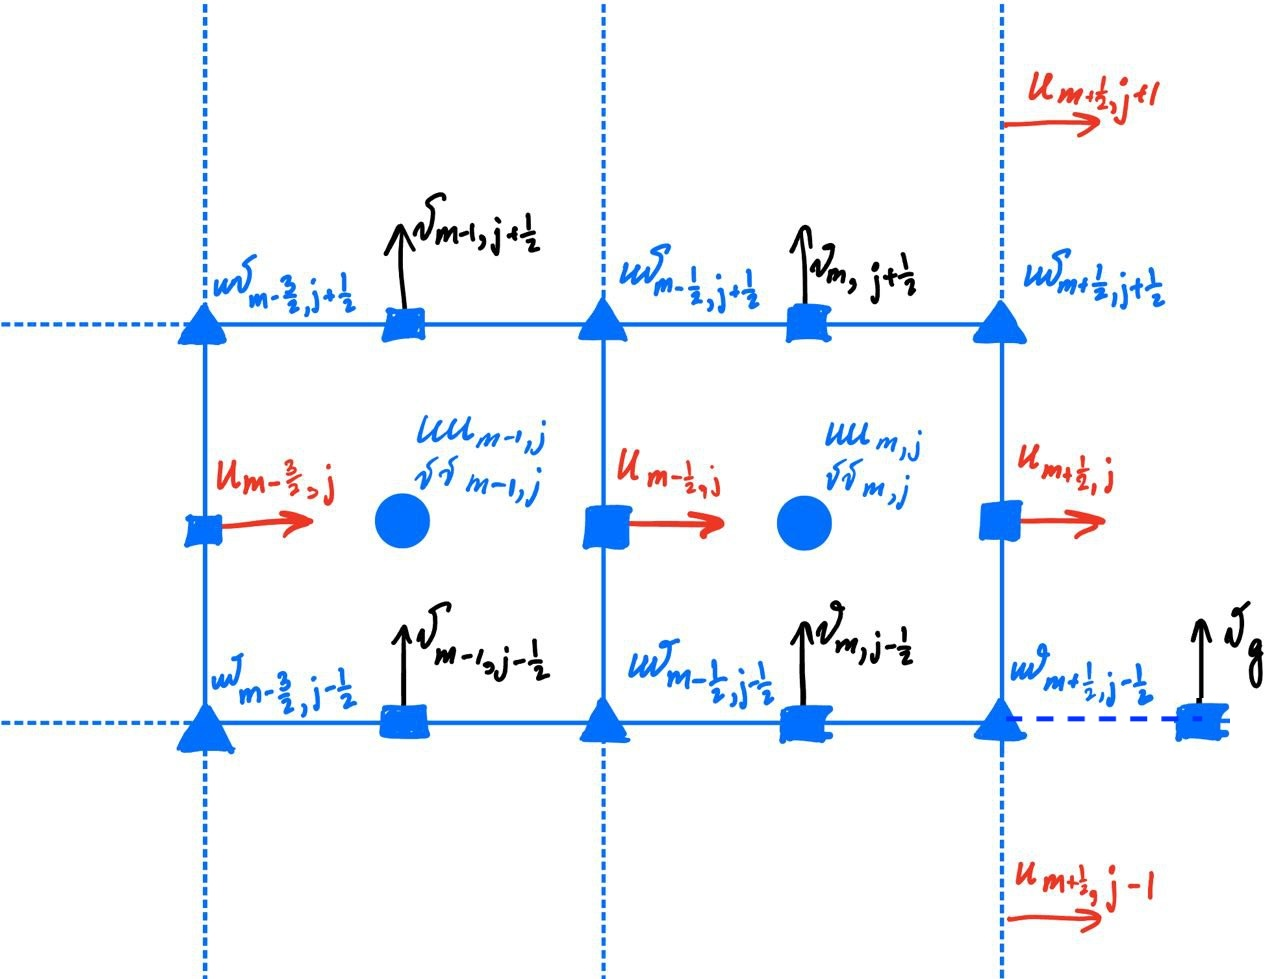
\includegraphics[width=0.55\paperwidth]{ADV-right}
  }
  \caption{Right boundary advection ($m=M,n=N$).}\label{fig:ADV-right}
\end{figure}




%%%%%%%%%%%%%%%%%%%%%%%%%%%%%%%%%%%%%%%%%%%%%%
\subsection{Divergence}\label{subsec:divergence}

One of the advantages of the staggered grid is that the discrete divergence $D$ and gradient $G$ operators are equal to the negative transpose of each other. 
%Our goal is to eliminate the pressure from the system, \cref{subsec:curl} will explain the use of this property in detail. 
In this section, we will show one side of why this identity is true (the other part could be found in \cref{subsec:gradient}).
The second line of \cref{eqn:NSE-dsm-bl-system-schemes} reads:
\begin{equation}\label[pluralequation]{eqn:divergence-modification}
\begin{gathered}
\hat{D}\boldsymbol{v}=\hat{bc}_2,\\
\left[ 
\begin{array}{ll}
\hat{D}_x & \hat{D}_y 	
\end{array}
\right]\left[\begin{array}{l}
u\\
v
\end{array}
\right]=\hat{bc}_2
, \\
\frac{1}{\Delta x} D_x u+\frac{1}{\Delta y} D_y v=\hat{bc}_2, \\
\frac{1}{\Delta _{xy}}\left[\begin{array}{ll}
D_x & D_y
\end{array}\right]\left[\begin{array}{l}
u \Delta y \\
v \Delta x
\end{array}\right]=\frac{1}{\Delta _{xy}} D q=\hat{bc}_2,
\end{gathered}
\end{equation}
where vector $q=\left[\begin{array}{l}
u \Delta y \\
v \Delta x
\end{array}\right]$ is referred to as velocity flux, and the matrix $D=[D_x D_y]$ is the divergence matrix of integer coefficients. Matrix
\begin{equation}\label{eqn:delta-xy}
	\frac{1}{\Delta _{xy}}=
	\begin{bmatrix}{}
		\frac{1}{\Delta x_1\Delta y_1}		&0	&\dots	&0\\
		0		&\frac{1}{\Delta x_2\Delta y_1}	&\dots	&0\\
		\vdots		&\vdots	&\ddots	&\vdots\\
		0		&0	&\dots	&\frac{1}{\Delta x_M\Delta y_N}
	\end{bmatrix}
\end{equation}
is $MN\times MN$ diagonal matrix with entries corresponding to the inverse volumes of cells. 

The second-order central difference scheme employed in the construction of $D$ is consistent with other spatial schemes used in this paper. Continuity equation for the cell centre that lies in a finite volume $V_{i,j}$ is expressed as
\begin{equation*}
	\left(\frac{\partial u}{\partial x} + \frac{\partial v}{\partial y}\right)_{i,j}=0,
\end{equation*}
which can be discretized at cell centre $i,j$ using central difference schemes into
\begin{equation*}
  \frac{u_{i+\frac{1}{2},j} - u_{i-\frac{1}{2},j}}{\Delta x_i}+  \frac{v_{i,j+\frac{1}{2}} - v_{i,j-\frac{1}{2}}}{\Delta y_j}=0.
\end{equation*}

\begin{figure}[H] % here, bottom, top
  \centering{
  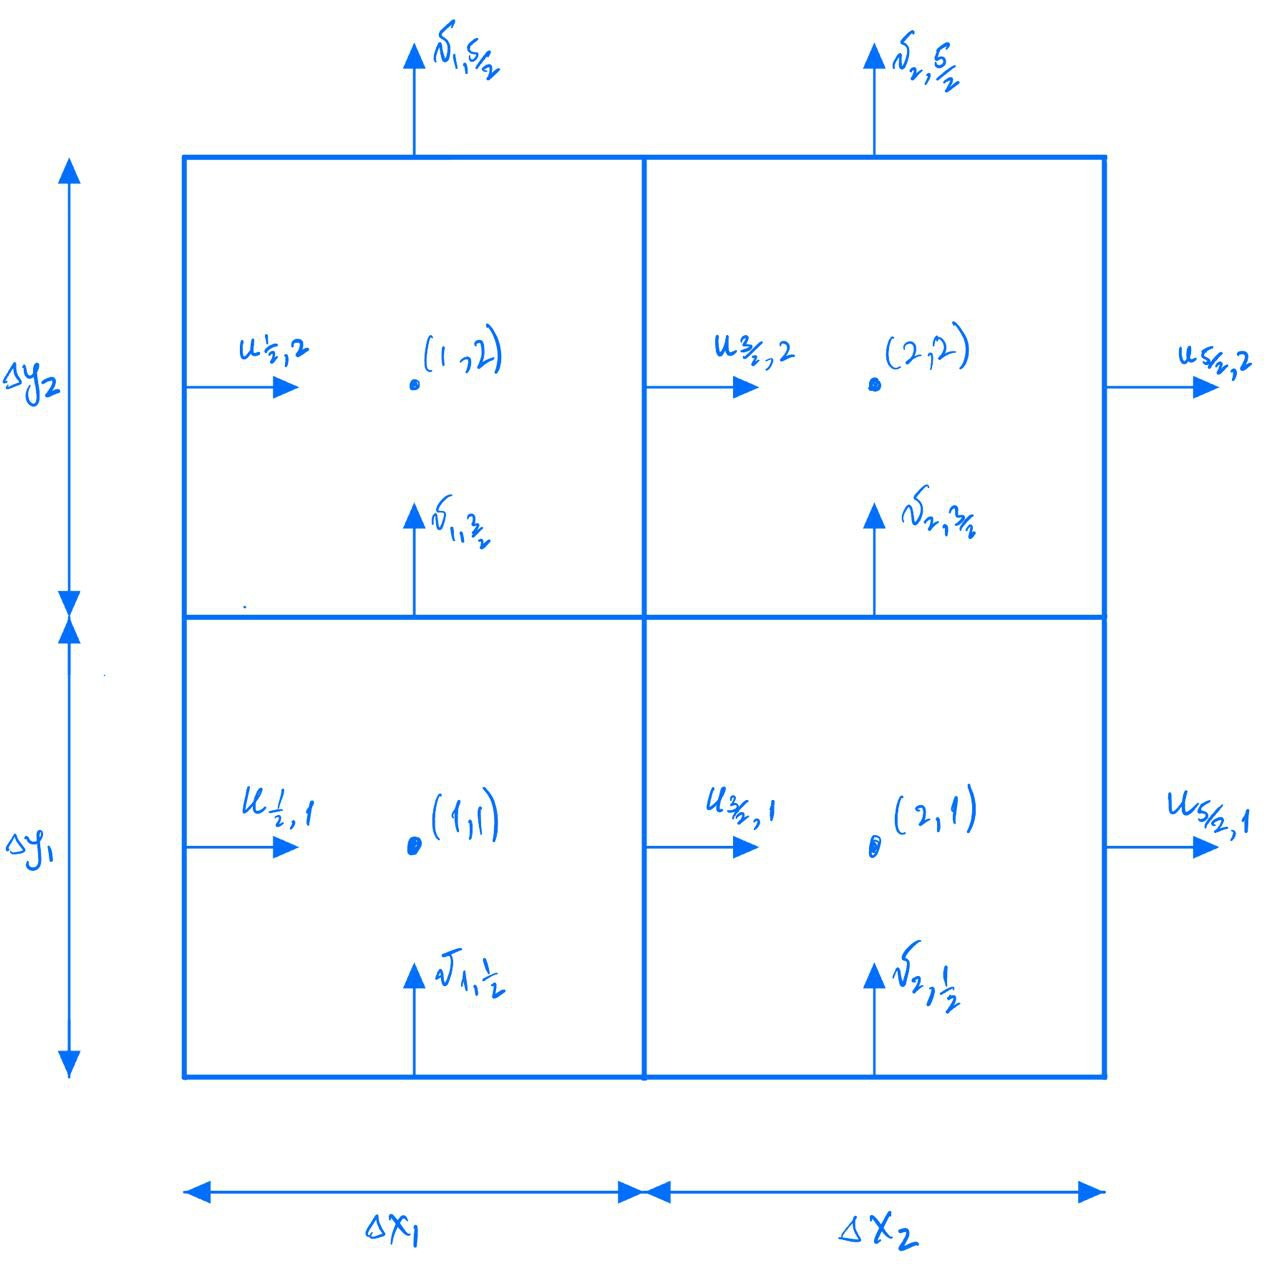
\includegraphics[width=0.55\paperwidth]{D-example-2x2}
  }
  \caption{$2\times 2$ grid example for divergence operator.}\label{fig:D-example-2x2}
\end{figure}

To provide a good visual example, consider $2 \times 2$ grid as in \cref{fig:D-example-2x2} with the same boundary conditions as in \cref{eqs:NSE-dsm-bl}. The partial derivatives of divergence operator evaluated at cell centres $V_{i,j}$ are: 
$$
\begin{aligned}
& V_{1,1}: \frac{u_{\frac{3}{2},1}-u_{\frac{1}{2},1}}{\Delta x_1}+\frac{v_{1,\frac{3}{2}}-v_{1,\frac{1}{2}}}{\Delta y_1}=0, \\
& V_{1,2}: \frac{u_{\frac{5}{2},1}-u_{\frac{3}{2},1}}{\Delta x_2}+\frac{v_{2,\frac{3}{2}}-v_{2,\frac{1}{2}}}{\Delta y_1}=0, \\
& V_{2,1}: \frac{u_{\frac{3}{2},2}-u_{\frac{1}{2},2}}{\Delta x_1}+\frac{v_{1,\frac{5}{2}}-v_{1,\frac{3}{2}}}{\Delta y_2}=0, \\
& V_{2,2}: \frac{u_{\frac{5}{2},2}-u_{\frac{3}{2},2}}{\Delta x_2}+\frac{v_{2,\frac{5}{2}}-v_{2,\frac{3}{2}}}{\Delta y_2}=0 .
\end{aligned}
$$

After applying the same operations as in \cref{eqn:divergence-modification} to discrete continuity equations from above, we obtain the following system
\begin{equation}\label[system]{eqn:divergence-matrix}
\operatorname{diag}\left(\begin{array}{cccc}
\frac{1}{\Delta x_1 \Delta y_1} \\
\frac{1}{\Delta x_2 \Delta y_1} \\
\frac{1}{\Delta x_1 \Delta y_2} \\
\frac{1}{\Delta x_2 \Delta y_2}
\end{array}\right)
\left[ \begin{array}{rrrrrrrrrrrr}
-1 & 1 & 0 & 0 & 0 & 0 & -1 & 0 & 1 & 0 & 0 & 0 \\
0 & -1 & 1 & 0 & 0 & 0 & 0 & -1 & 0 & 1 & 0 & 0 \\
0 & 0 & 0 & -1 & 1 & 0 & 0 & 0 & -1 & 0 & 1 & 0 \\
0 & 0 & 0 & 0 & -1 & 1 & 0 & 0 & 0 & -1 & 0 & 1
\end{array} \right]
\left[\begin{array}{l}
u_{\frac{1}{2},1} \Delta y_1 \\
u_{\frac{3}{2},1} \Delta y_1 \\
u_{\frac{5}{2},1} \Delta y_1 \\
u_{\frac{1}{2},2} \Delta y_2 \\
u_{\frac{3}{2},2} \Delta y_2 \\
u_{\frac{5}{2},2} \Delta y_2 \\
v_{1,\frac{1}{2}} \Delta x_1 \\
v_{2,\frac{1}{2}} \Delta x_2 \\
v_{1,\frac{3}{2}} \Delta x_1 \\
v_{2,\frac{3}{2}} \Delta x_2	 \\
v_{1,\frac{5}{2}} \Delta x_1 \\
v_{2,\frac{5}{2}} \Delta x_2 \\
\end{array}\right]=
\begin{bmatrix}{}
0 \\
0 \\
0 \\
0
\end{bmatrix}.
\end{equation}

\cref{eqn:divergence-matrix} in general case is written as $\frac{1}{\Delta_{xy}} D q=\hat{bc}_2$.
We have used boundary velocities in vector $\boldsymbol{v}$ (as recommended by Chang~\cite{Chang:2002}) to eliminate any explicit boundary condition treatment of the incompressibility constraint. The divergence matrix $D$ contains zeros and $\pm1$ as shown in \cref{eqn:divergence-matrix}.


%%%%%%%%%%%%%%%%%%%%%%%%%%%%%%%%%%%%%%%%%%%%%%
\subsection{Gradient}\label{subsec:gradient} 

The pressure gradients are computed at the same coordinates as the unknown velocities in \cref{eqn:nse-matrix}. In this section, we will demonstrate that the discrete gradient and divergence operators comply with
\begin{equation}\label{eqn:g-dt}
  {G}=-{D^T}
\end{equation}
on staggered/MAC grids by construction. 

As an illustrative example, we may consider gradient operator on $2\times 2$ grid as in \cref{fig:G-example-2x2} with boundary conditions from \cref{eqs:NSE-dsm-bl}. The normal distances between the computational domain and virtual pressure values located outside of it are considered to be infinitesimally small~\cite{Chang:2002}.  It is required to determine the pressure gradients across each unknown velocity (square nodes on \cref{fig:G-example-2x2}):

\begin{figure}[H] % here, bottom, top
  \centering{
  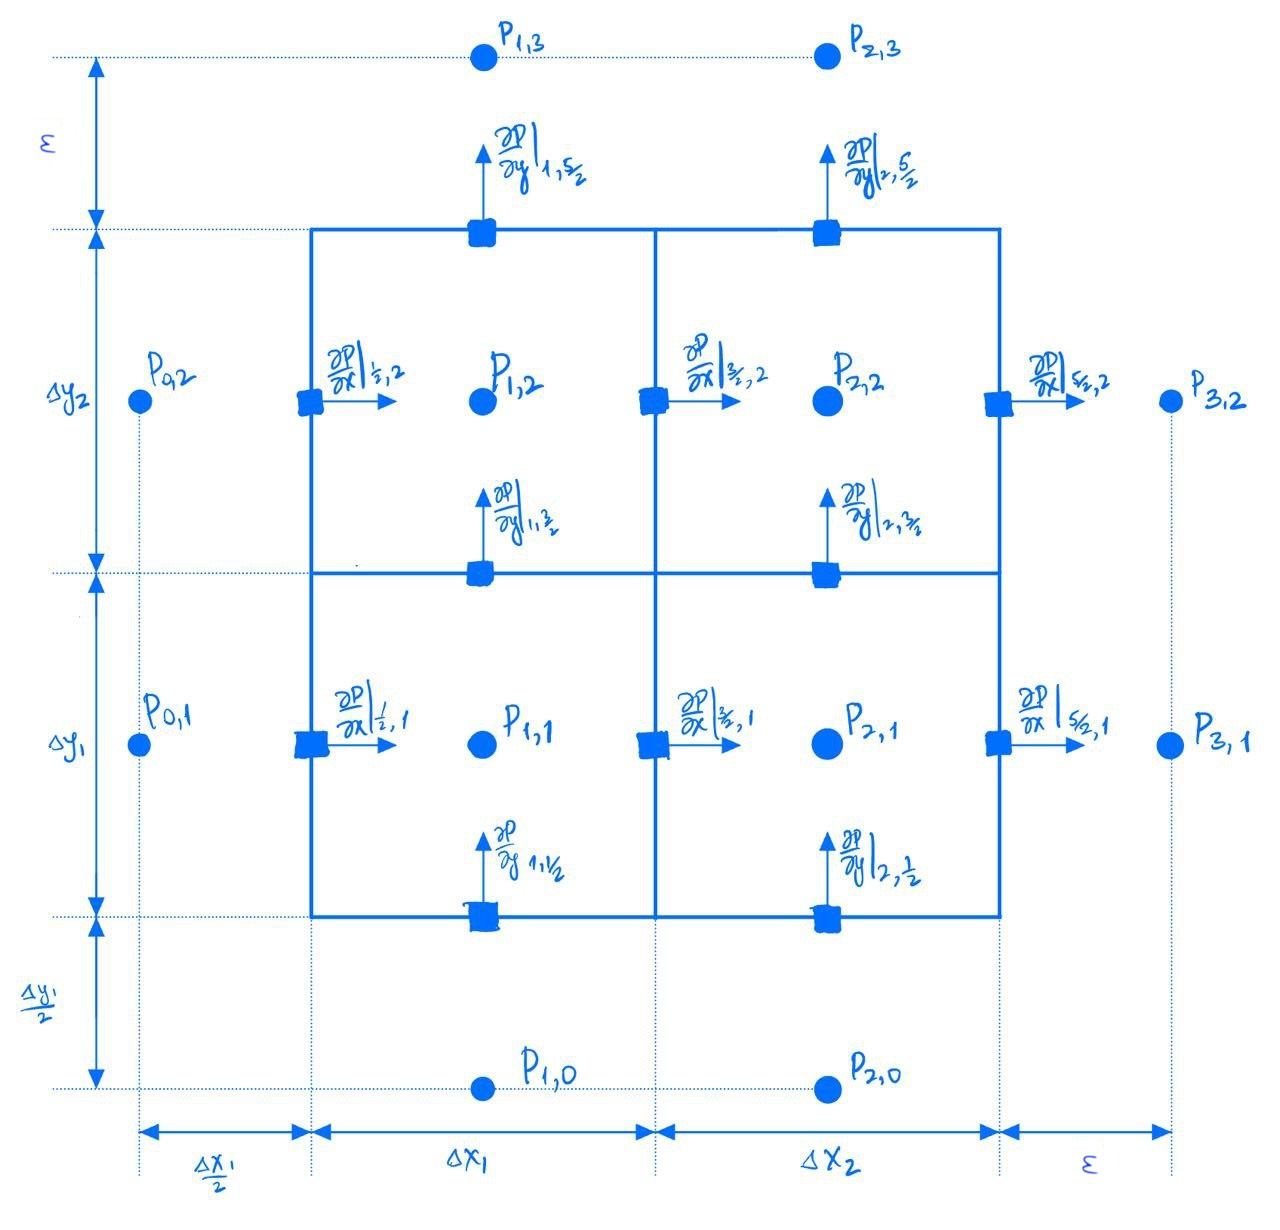
\includegraphics[width=0.55\paperwidth]{G-example-2x2}
  }
  \caption{$2\times 2$ grid example for gradient operator ($\varepsilon\to 0$).}\label{fig:G-example-2x2}
\end{figure}

$$
\begin{aligned}
u_{\frac{1}{2},1} & : \frac{2}{\Delta x_1}\left(p_{1,1}-p_{0,1}\right), \\
u_{\frac{3}{2},1} & : \frac{2}{\Delta x_1+\Delta x_2}\left(p_{2,1}-p_{1,1}\right), \\
u_{\frac{5}{2},1} & : \frac{2}{\Delta x_2}\left(p_{3,1}-p_{2,1}\right), \\
u_{\frac{1}{2},2} & : \frac{2}{\Delta x_1}\left(p_{1,2}-p_{0,2}\right), \\
u_{\frac{3}{2},2} & : \frac{2}{\Delta x_1+\Delta x_2}\left(p_{2,2}-p_{1,2}\right), \\
u_{\frac{5}{2},2} & : \frac{2}{\Delta x_2}\left(p_{3,2}-p_{2,2}\right), \\
v_{1,\frac{1}{2}} & : \frac{2}{\Delta y_1}\left(p_{1,1} - p_{1,0}\right),\\
v_{2,\frac{1}{2}} & : \frac{2}{\Delta y_1}\left(p_{2,1} - p_{2,0}\right),\\
v_{1,\frac{3}{2}} & : \frac{2}{\Delta y_1+\Delta y_2}\left(p_{1,2}-p_{1,1}\right), \\
v_{2,\frac{3}{2}} & : \frac{2}{\Delta y_1+\Delta y_2}\left(p_{2,2}-p_{2,1}\right), \\
v_{1,\frac{5}{2}} & : \frac{2}{\Delta y_2}\left(p_{1,3} - p_{1,2}\right),\\
v_{2,\frac{5}{2}} & : \frac{2}{\Delta y_2}\left(p_{2,3} - p_{2,2}\right).
\end{aligned}
$$

The next step is to rewrite the above expressions in matrix form using the pressure boundary conditions. The resultant system of linear equations then becomes
\begin{equation}\label[system]{eqn:gradient-matrix}
\operatorname{diag}\left(\begin{array}{cccccc}
\frac{2}{\Delta x_1} \\
\frac{2}{\Delta x_1+\Delta x_2} \\
\frac{2}{\Delta x_2} \\
\frac{2}{\Delta x_1} \\
\frac{2}{\Delta x_1+\Delta x_2} \\
\frac{2}{\Delta x_2}\\
\frac{2}{\Delta y_1}\\
\frac{2}{\Delta y_1}\\
\frac{2}{\Delta y_1+\Delta y_2}\\
\frac{2}{\Delta y_1+\Delta y_2}\\
\frac{2}{\Delta y_2}\\
\frac{2}{\Delta y_2}
\end{array}\right)
\left(\left[
\begin{array}{rrrr}
1 & 0 & 0 & 0 \\
-1 & 1 & 0 & 0 \\
0 & -1 & 0 & 0 \\
0 & 0 & 1 & 0 \\
0 & 0 & -1 & 1 \\
0 & 0 & 0 & -1 \\
1 & 0 & 0 & 0 \\
0 & 1 & 0 & 0 \\
-1 & 0 & 1 & 0 \\
0 & -1 & 0 & 1 \\
0 & 0 & -1 & 0 \\
0 & 0 & 0 & -1
\end{array}
\right]
\begin{bmatrix}{}
  p_{1,1} \\
  p_{2,1} \\
  p_{1,2} \\
  p_{2,2} 
\end{bmatrix}
+\left[\begin{array}{c}
p_{0,1} \\
0 \\
p_{3,1} \\
p_{0,2} \\
0 \\
p_{3,2} \\
p_{1,0} \\
p_{2,0} \\
0 \\
0 \\
p_{1,3} \\
p_{2,3}
\end{array}\right]\right),
\end{equation}
which can be rewritten in compact format as
$$
\nabla p+b c_p \Longleftrightarrow 
\hat{M}^{-1} \left(\hat{G}\left[\begin{array}{c}
p_{1,1} \\
p_{2,1} \\
\vdots \\
p_{M,N}
\end{array}\right]+bc_p\right),
$$
where $\hat{M}^{-1}$ is the diagonal matrix containing the inverse distances between neighbouring pressure coordinates; ${G}$ is integer gradient matrix and $[p_{1,1},p_{2,1},...,p_{M,N}]^T$ is the vector of pressure values at the cell centres. There are some pressure BC values in ${bc}_p$ since there is a pressure gradient that has to be computed across the boundary. It can be observed from \cref{eqn:divergence-matrix,eqn:gradient-matrix} that \cref{eqn:g-dt} holds and the general case is true by construction. 

Lastly, it is worth mentioning that pressure values at the boundaries with known velocities (inlet and wall) are not needed. The reason is that after constructing all momentum equations the corresponding rows are replaced by zeroes.



\subsection{Curl operator and pressure elimination}\label{subsec:curl}

The goal of this subsection is to show how unknown pressure variables can be eliminated from \cref{eqn:nse-normalized} similarly to \cref{sec:vorticity-streamfunction}. Publications of Chang~\cite{Chang:2002} and Hall~\cite{Hall:1980} use the idea that in \cref{eqn:nse-normalized} matrix $D$ is wider than tall, hence it defines a nullspace which we denote as $C$. 

The number of rows in the nullspace $C$ is equal to the number of momentum equations for all the velocities. In two dimensions $C$ has $N_n$ columns, which is equal to the number of the nodes in the grid, whereas in three dimensions the nullspace has $N_e$ columns being the number of edges.

In the two-dimensional case, the matrix $C$ has two non-zero elements in each row ($+1$ and $-1$). The $+1$ value corresponds to the node $90^\circ$ from the normal velocity vector, whereas $-1$ corresponds to the node $-90^\circ$ from the normal velocity vector.  For three dimensional case see Chang~\cite{Chang:2002}.

\begin{figure}[H] % here, bottom, top
  \centering{
  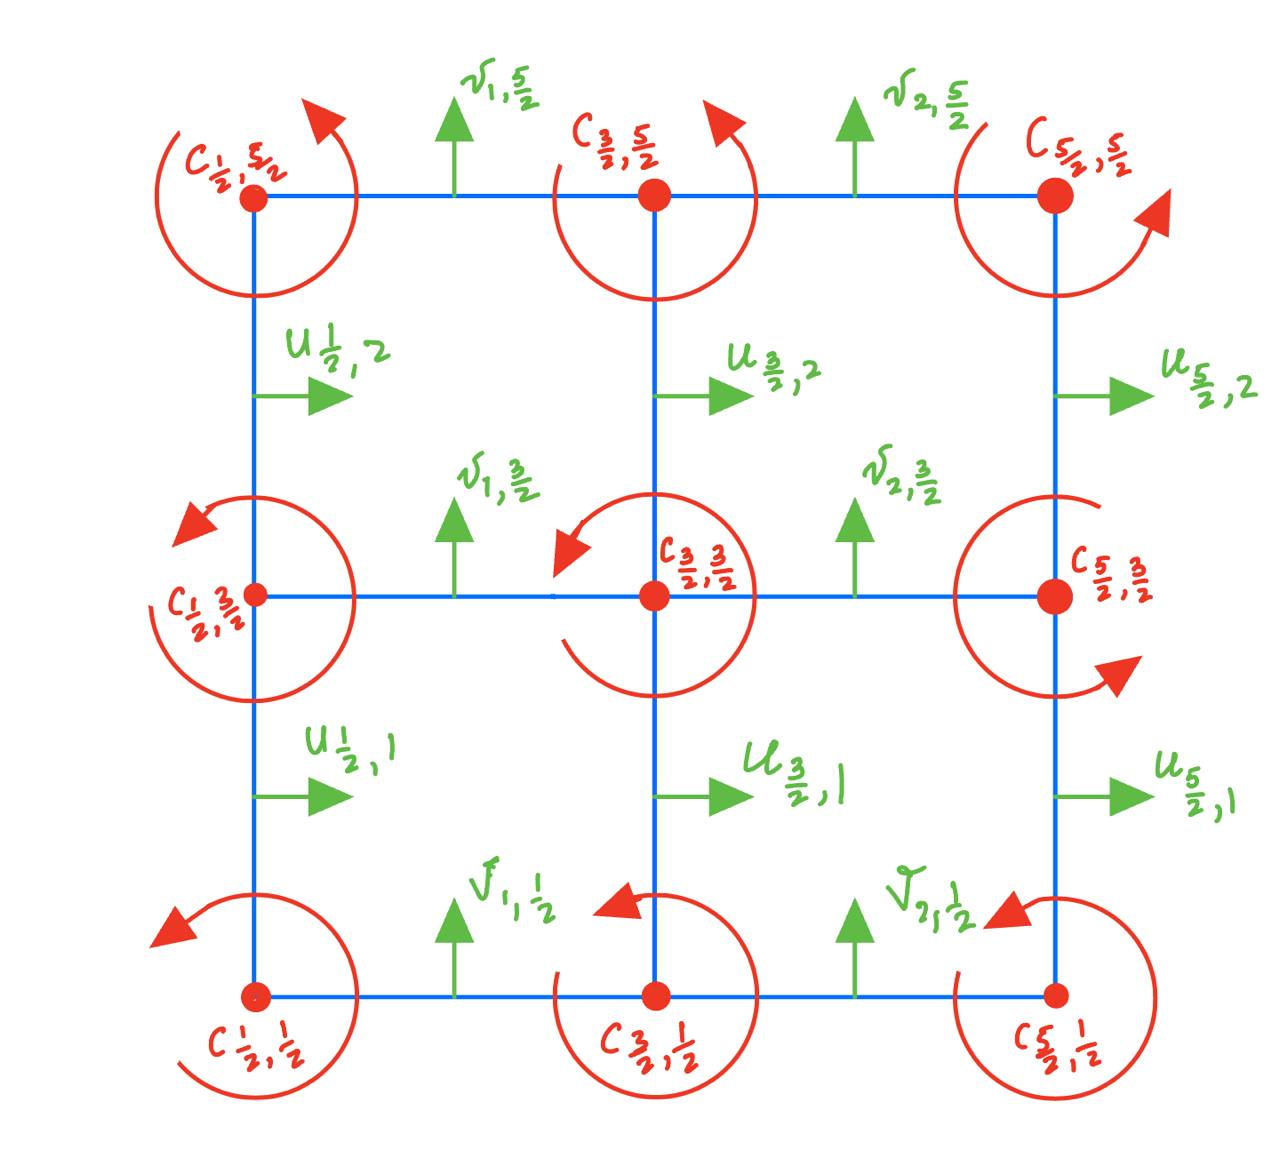
\includegraphics[width=0.40\paperwidth]{C-example-2x2}
  }
  \caption{$2\times 2$ example for $C$ matrix.}\label{fig:C-example-2x2}
\end{figure}
A more intuitive way of constructing the matrix $C$ relies on the utilization of counterclockwise vorticity around the nodes within the domain (\cref{fig:C-example-2x2}). If the direction of the velocity vector on the adjacent face aligns with the vorticity's direction, +1 is assigned to the corresponding row; conversely, -1 is assigned in the case of opposite directions of velocity and vorticity. After applying the above procedure to all nodes we obtain
\begin{equation}
C=\left[
\begin{array}{rrrrrrrrr}
-1 & 0 & 0 & 1 & 0 & 0 & 0 & 0 & 0 \\
0 & -1 & 0 & 0 & 1 & 0 & 0 & 0 & 0 \\
0 & 0 & -1 & 0 & 0 & 1 & 0 & 0 & 0 \\
0 & 0 & 0 & -1 & 0 & 0 & 1 & 0 & 0 \\
0 & 0 & 0 & 0 & -1 & 0 & 0 & 1 & 0 \\
0 & 0 & 0 & 0 & 0 & -1 & 0 & 0 & 1 \\
1 & -1 & 0 & 0 & 0 & 0 & 0 & 0 & 0 \\
0 & 1 & -1 & 0 & 0 & 0 & 0 & 0 & 0 \\
0 & 0 & 0 & 1 & -1 & 0 & 0 & 0 & 0 \\
0 & 0 & 0 & 0 & 1 & -1 & 0 & 0 & 0 \\
0 & 0 & 0 & 0 & 0 & 0 & 1 & -1 & 0 \\
0 & 0 & 0 & 0 & 0 & 0 & 0 & 1 & -1
\end{array}
\right].
\end{equation}
%Matrix $C$ has dimensions corresponding to unknown velocities times the number of nodes around which these velocities revolve. % already mentioned at the beginning

The desired product then becomes $DC=0$. $D=-G^T$ (derived in \cref{subsec:divergence,subsec:gradient}) leads to important property $(DC)^T=C^TD^T=-C^TG=0$. Premultiplying momentum equation from \cref{eqn:nse-normalized} by $C^T$ creates $C^TGp=0$ term, which  eliminates the pressure from our system, however, leaves pressure boundary conditions which we will discuss in \cref{sec:artificial-bc}.

In order to make use of efficient solvers, the matrix $C^TA$ can be made symmetric if multiplied by $C$ from the right. The matrix $C^TC$ is equivalent to Laplacian (Chang~\cite{Chang:2002} uses $RC$ notation), whereas $C^TLC$ is equivalent to symmetric biharmonic operator of streamfunction $\psi$ as in \cref{eqn:biharmonic-streamfunction}. Laplacian operator discretization will be discussed in the following \cref{sec:laplacian}.



\subsection{Laplacian}\label{sec:laplacian}
As per \cref{eqn:NSE-dsm-bl-system-schemes}, it is required to approximate implicit viscous terms spatially. In order to obtain the discrete operator acting on a velocity vector we will rewrite Laplacian as a block matrix:
\begin{equation*}
	\hat L=
	\begin{bmatrix}
  \hat{L}^u_{xx}+\hat{L}^u_{yy} & 0 \\
  0 & \hat{L}^v_{xx}+\hat{L}^v_{yy}
\end{bmatrix}.
\end{equation*}

Each pair of the matrices $\hat{L}^u_{xx},\hat{L}^v_{xx}$ and $\hat{L}^u_{yy},\hat{L}^v_{yy}$ will be equal on a uniform, but different on non-uniform grids. These matrices are computed in a similar manner. Below we will discuss how the Laplacian matrix is constructed on different parts of the grid. We will only display inner, bottom and left part discretizations in this section, the rest will be derived in artificial boundary conditions \cref{sec:artificial-bc}.

\subsubsection{Inner part.}\label{sec:laplacian-inner}
The uniform grid refinement $\Delta x_{i+1}=k_x\Delta x_i,\Delta y_{j+1}=k_y\Delta y_j$ makes the order of the scheme consistent throughout the whole domain. Without loss of generality, let us compute $\hat{L}^u_{xx}$. The other three matrices can be constructed in the same way. The power series of of $u_{i-\frac{1}{2}\pm 1,j}$ at nodes $x_{i - \frac{1}{2}\pm 1}$ with respect to $u_{i - \frac{1}{2},j}$ at node $x_{i-\frac{1}{2}}$ are:
\begin{equation}\label{eqn:Taylor right} 
	u_{i-\frac{1}{2}+1,j}=u_{i-\frac{1}{2},j}+\left.\frac{\partial u}{\partial x}\right|_{i-\frac{1}{2},j}\left(x_{i-\frac{1}{2}+1}-x_{i-\frac{1}{2}}\right)+\frac{1}{2}\left.\frac{\partial^2 u}{\partial x^2}\right|_{i-\frac{1}{2},j}\left(x_{i-\frac{1}{2}+1}-x_{i-\frac{1}{2}}\right)^2+O\left(\Delta x^3\right),
\end{equation}
\begin{equation}\label{eqn:Taylor left} 
	u_{i-\frac{1}{2}-1,j}=u_{i-\frac{1}{2},j}+\left.\frac{\partial u}{\partial x}\right|_{i-\frac{1}{2},j}\left(x_{i-\frac{1}{2}-1}-x_{i-\frac{1}{2}}\right)+\frac{1}{2}\left.\frac{\partial^2 u}{\partial x^2}\right|_{i-\frac{1}{2},j}\left(x_{i-\frac{1}{2}-1}-x_{i-\frac{1}{2}}\right)^2+O\left(\Delta x^3\right).
\end{equation}
We can combine \cref{eqn:Taylor left,eqn:Taylor right} by cancelling the first derivative, which will result in
\begin{align}\label{eqn:laplacian-discretization-non-uniform-dx}
\left.\frac{\partial^2 u}{\partial x^2}\right|_{i-\frac{1}{2},j} & \approx \frac{u_{i-\frac{1}{2}+1,j}\left(x_{i-\frac{1}{2}}-x_{i-\frac{1}{2}-1}\right)-u_{i-\frac{1}{2},j}\left(x_{i-\frac{1}{2}+1}-x_{i-\frac{1}{2}-1}\right)+u_{i-\frac{1}{2}-1,j}\left(x_{i-\frac{1}{2}+1}-x_{i-\frac{1}{2}}\right)}{\left(\frac{x_{i-\frac{1}{2}+1}-x_{i-\frac{1}{2}-1}}{2}\right)\left(x_{i-\frac{1}{2}}-x_{i-\frac{1}{2}-1}\right)\left(x_{i-\frac{1}{2}+1}-x_{i-\frac{1}{2}}\right)}+O(\Delta x)\notag\\
& \approx u_{i-\frac{1}{2}+1}\frac{1}{h_c h_e} - u_{i-\frac{1}{2}} \frac{2}{h_w h_e}+ u_{i-\frac{1}{2}-1}\frac{1}{h_c h_w} + O(\Delta x),
\end{align}
where $h_w=x_{i-\frac{1}{2}}-x_{i-\frac{1}{2}-1},h_c = \frac{x_{i-\frac{1}{2}+1}-x_{i-\frac{1}{2}-1}}{2}, h_e = x_{i-\frac{1}{2}+1}-x_{i-\frac{1}{2}}$ (cf. \cref{fig:luxx-inner}). The coefficients after the velocity components are then placed into the $\hat{L}^u_{xx}$ matrix. The order of this approximation becomes $2^{\text {nd }}$ on uniform grids. 

\begin{figure}[H] % here, bottom, top
  \centering{
  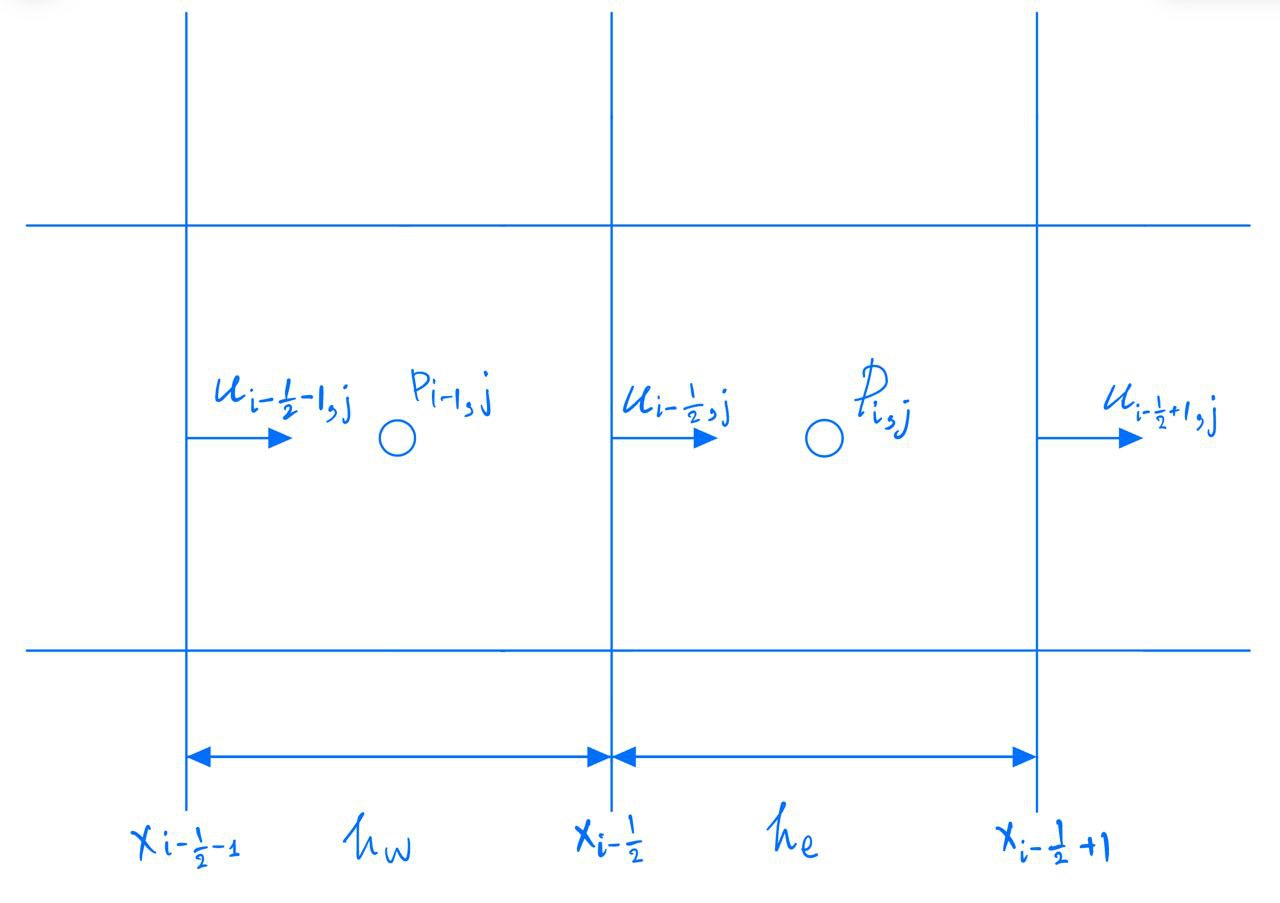
\includegraphics[width=0.45\paperwidth]{Luxx}
  }
  \caption{$\hat{L}^u_{xx}$ inner part.}\label{fig:luxx-inner}
\end{figure}
%The discretization for such grids is reduced to 
%\begin{equation}\label{eqn: second derivative uniform}
%\left(\frac{\partial^2 u}{\partial x^2}\right)_i \approx \frac{u_{i+1}-2 u_i+u_{i-1}}{(\Delta x)^2} + O(\Delta x^2).
%\end{equation}



\subsubsection{Left boundary.}\label{sec:laplacian-left}
The exact value at the left boundary (normal velocity $u_{\frac{1}{2},j}$ on \cref{fig:luxx-left}) is given as a Dirichlet boundary condition. The value of $u_{\frac{1}{2},j}$ is known, therefore it is possible to move it to the vector $\hat{bc}_1$. Discretization of Laplacian operator of $u_{\frac{1}{2}+1,j}$ term is then
\begin{equation}\label{eqn:laplacian-discretization-u-left-deltax}
\left.\frac{\partial^2 u}{\partial x^2}\right|_{\frac{1}{2}+1,j}=
\frac{
	u_{\frac{1}{2},j}\left(\Delta x_2\right)
	+u_{\frac{1}{2}+1,j}\left(-[\Delta x_1 + \Delta x_2]\right)
	+u_{\frac{1}{2}+2,j}\left(\Delta x_1\right)}
	{\Delta x_1 \frac{\Delta x_1+\Delta x_2}{2} \Delta x_2}
	,
\end{equation}
which in terms of $h_w,h_c,h_e$ and corresponding row of $\hat{L}_{xx}^u$ becomes
\begin{equation}\label{eqn:laplacian-discretization-u-left}
\left.\hat{L}_{xx}^u\right|_{\frac{1}{2}+1,j}+\left.\hat{L}^u_{\hat{bc}_1}\right|_{\frac{1}{2}+1,j}\iff
	\left[\frac{
		u_{\frac{1}{2}+1,j}\left(-2h_c\right)
		+u_{\frac{1}{2}+2,j}\left(h_w\right)
	}
	{h_e h_c h_w}\right]
	+\left[\frac{u_{\frac{1}{2},j}\left(h_e\right)}{h_e h_c h_w}\right],
\end{equation}
where $\hat{L}^u_{\hat{bc}_1}$ is contribution of boundary condition from $\hat{L}^u_{xx}$ to $\hat{bc}_1$. We treat normal boundary conditions explicitly in momentum equations (Chang~\cite{Chang:2002} suggests that only incompressibility constraint to be not treated explicitly). Therefore, there is no need to discretize Laplacian at $u_{\frac{1}{2},j}$. 

\begin{figure}[H] % here, bottom, top
  \centering{
  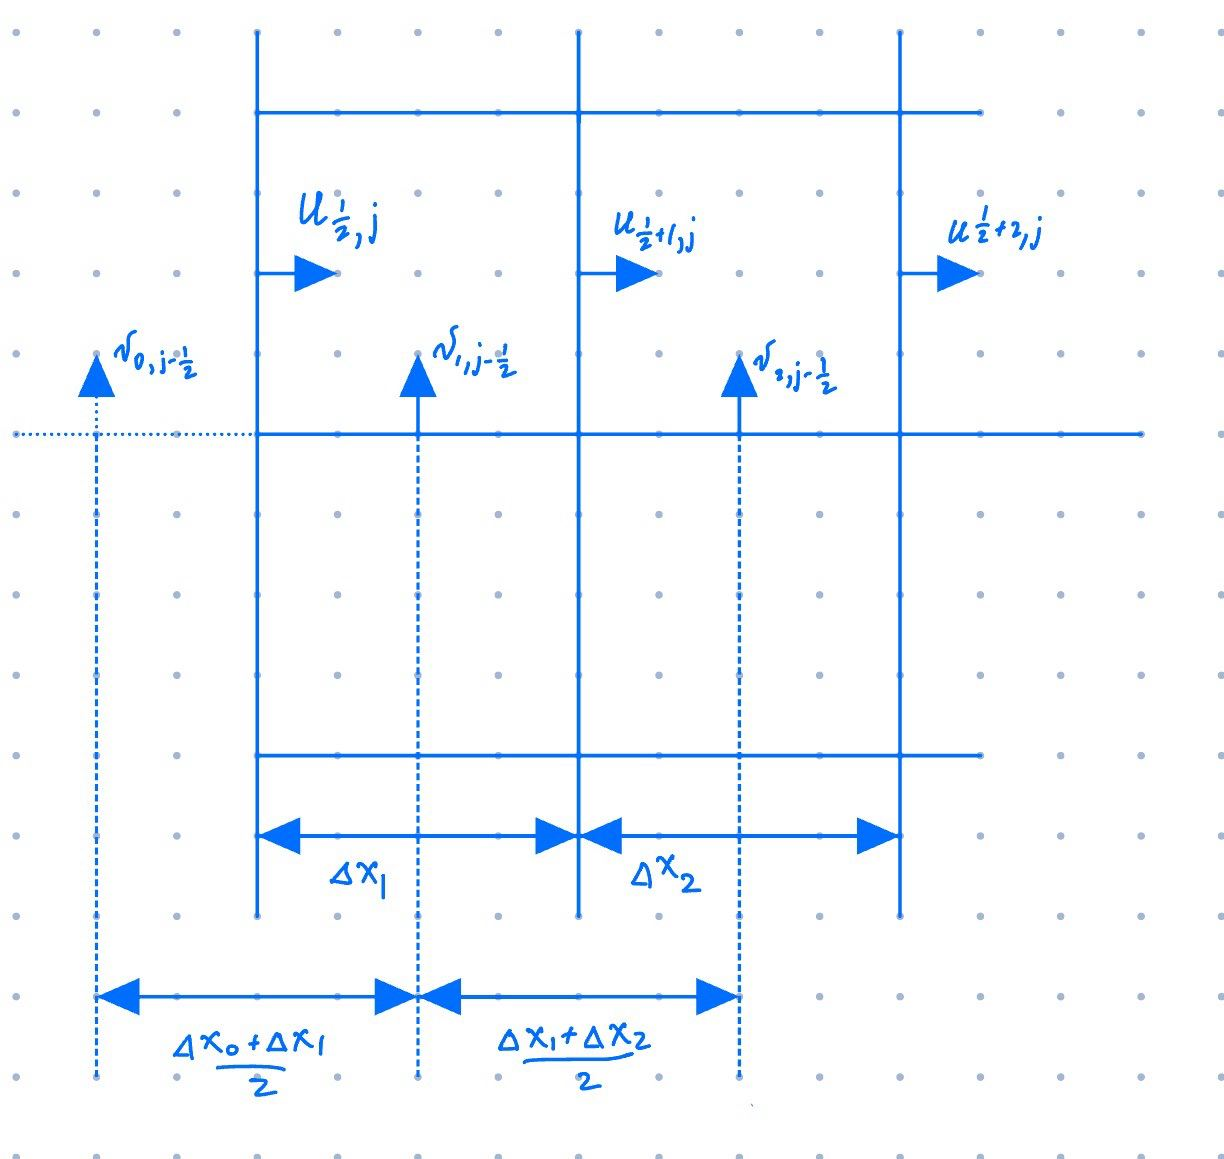
\includegraphics[width=0.45\paperwidth]{Luxx-left}
  }
  \caption{$\hat{L}^u_{xx}$ at the left boundary.}\label{fig:luxx-left}
\end{figure}

In fact, it is possible to directly use one of the velocities directly from the boundary when computing Laplacian at $v_{1,j-\frac{1}{2}}$. 
However, the order of such a scheme will then be reduced due to the large ratio of distances between the neighbouring velocities. 
If, on the other hand, we introduce a ghost velocity $v_{0,j-\frac{1}{2}}$, we have the freedom to chose its coordinate.
The corresponding viscous term at $v_{1,j-\frac{1}{2}}$ component becomes
\begin{equation}\label{eqn:laplacian-discretization-v-left-deltax}
\left.\frac{\partial^2 v}{\partial x^2}\right|_{1,j-\frac{1}{2}}=
\frac{
	v_{0,j-\frac{1}{2}}\left(\frac{\Delta x_1 + \Delta x_2}{2}\right)
	+v_{1,j-\frac{1}{2}}\left(-\frac{\Delta x_1 + \Delta x_2}{2}-\frac{\Delta x_0 + \Delta x_1}{2}\right)
	+v_{2,j-\frac{1}{2}}\left(\frac{\Delta x_0 + \Delta x_1}{2}\right)
}
{\frac{\Delta x_1 + \Delta x_2}{2} \frac{\frac{\Delta x_1 + \Delta x_2}{2}+\frac{\Delta x_0 + \Delta x_1}{2}}{2} \frac{\Delta x_0 + \Delta x_1}{2}},
\end{equation}
applying $v_{0,j-\frac{1}{2}}=0$, using $h_e,h_c,h_w$ and writing $\hat{L}^v_{xx}$ with $\hat{L}^v_{\hat{bc}_1}$ leads to
\begin{equation}\label{eqn:laplacian-discretization-v-left}
\left.\hat{L}^v_{xx}\right|_{1,j-\frac{1}{2}}+\left.\hat{L}^v_{\hat{bc}_1}\right|_{1,j-\frac{1}{2}}\iff
\left[\frac{
	v_{1,j-\frac{1}{2}}\left(-2h_c\right)
	+v_{2,j-\frac{1}{2}}\left(h_e\right)
}
{h_e h_c h_w}\right]
+\left[0\right].
\end{equation}




\subsubsection{Bottom boundary.}\label{sec:laplaciat-bot}
Let us use \cref{eqn:laplacian-discretization-non-uniform-dx} and change the distances between velocities as in \cref{fig:luxx-bottom}. This leads to
\begin{equation}
\begin{aligned}
&\left.\frac{\partial^ 2 u}{\partial y^2}\right|_{i-\frac{1}{2},1}=u_{i-\frac{1}{2},2}\left(\frac{1}{h_n h_c}\right)+u_{i-\frac{1}{2},1}\left(\frac{-2}{h_n h_s}\right)+u_{i-\frac{1}{2},0}\left(\frac{1}{h_s h_c}\right).\\
\end{aligned}
\end{equation}

\begin{figure}[H] % here, bottom, top
  \centering{
  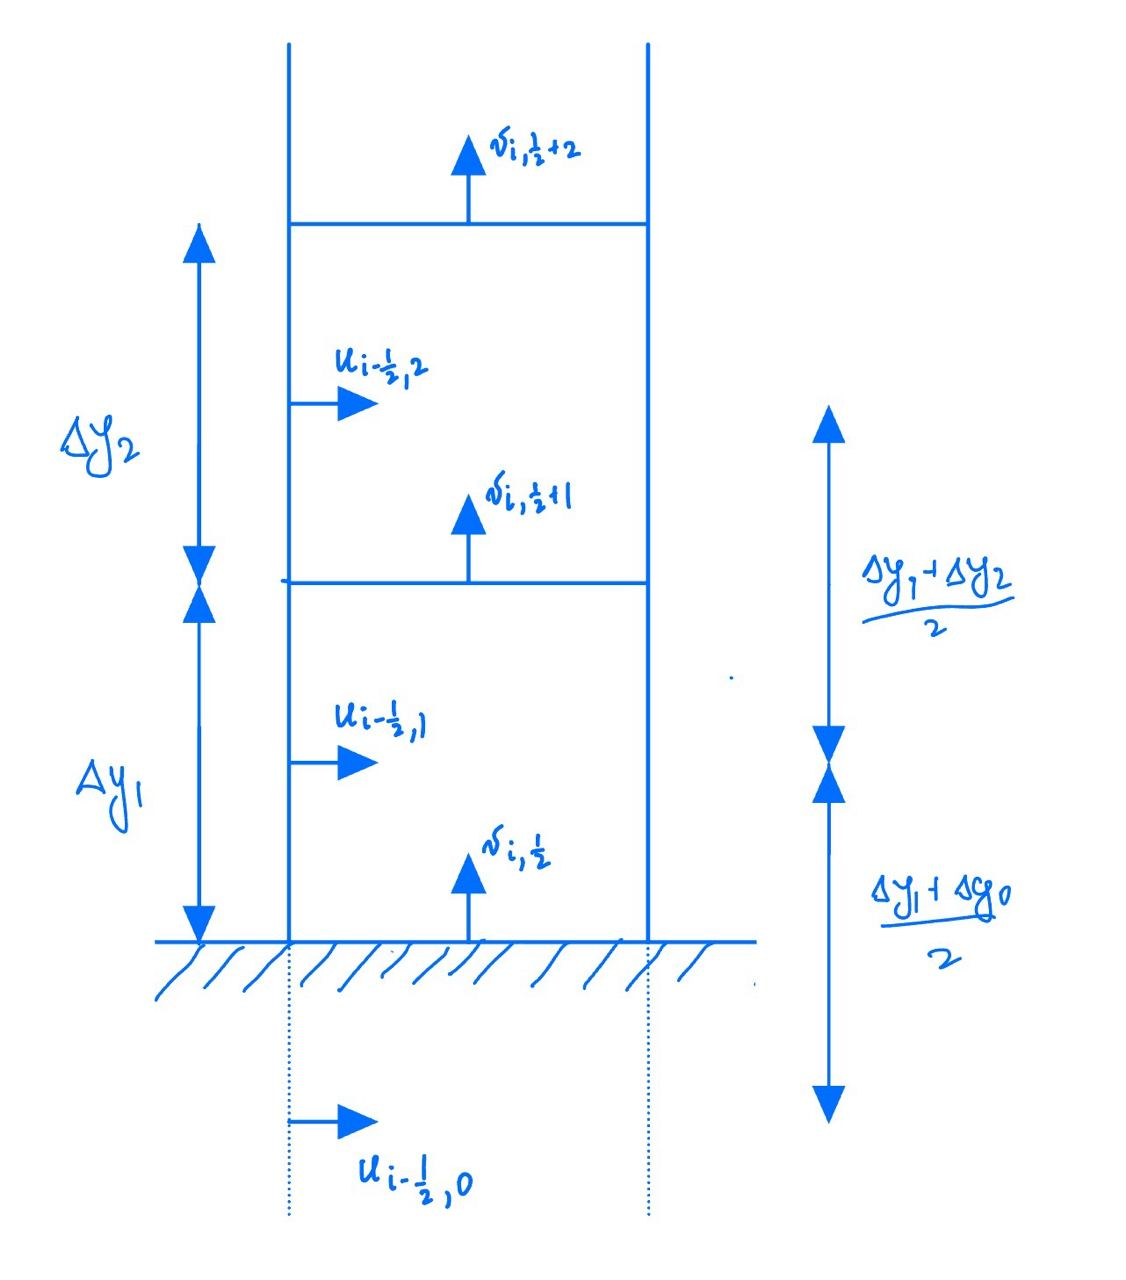
\includegraphics[width=0.45\paperwidth]{Luxx-bottom}
  }
  \caption{$\hat{L}^u_{yy}$ at the bottom boundary.}\label{fig:luxx-bottom}
\end{figure}

The position of $u_{i-\frac{1}{2},0}$ is not fixed, we can make the order of the scheme $O(\Delta y^2)$ if $h_s=\frac{\Delta y_1+\Delta y_0}{2}\equiv h_n=\frac{\Delta y_1+\Delta y_2}{2}$ when computing Laplacian for $u_{i-\frac{1}{2},1}$. Interpolation of velocity at the wall $u_{w} =\frac{u_{i-\frac{1}{2},1}+u_{i-\frac{1}{2},0}}{2}=0 \Rightarrow u_{i-\frac{1}{2},0}=-u_{i-\frac{1}{2},1}$, then
\begin{equation}\label{eqn:luyy-bot}
\begin{aligned}
\left.\frac{\partial^2 u}{\partial y^2}\right|_{i-\frac{1}{2},1} 
& =u_{i-\frac{1}{2},2}\left(\frac{1}{h_n h_c}\right)+u_{i-\frac{1}{2},1}\left(\frac{-2}{h_n h_s}+\frac{-1}{h_s h_c}\right) \\
& =u_{i-\frac{1}{2},2}\left(\frac{1}{h_n h_c}\right)+u_{i-\frac{1}{2},1}\left(\frac{-2 h_c- h_n}{h_s h_c h_n}\right).
\end{aligned}
\end{equation}
The coefficients from \cref{eqn:luyy-bot} are distributed into the $\hat{L}^u_{yy}$ matrix as
\begin{equation}
	\left.\hat{L}_{yy}^u\right|_{i-\frac{1}{2},1}+\left.\hat{L}^u_{\hat{bc}_1}\right|_{i-\frac{1}{2},1} \iff  \left[ u_{i-\frac{1}{2},2}\left(\frac{1}{h_n h_c}\right)+u_{i-\frac{1}{2},1}\left(\frac{-2 h_c- h_n}{h_s h_c h_n}\right)\right]+\left[0\right].
\end{equation}

Computation of Laplacian at $v_{i,\frac{1}{2}+1}$ can be performed similarly to the $\hat{L}_{xx}^u$ at the left boundary 
\begin{equation}
	\left.\hat{L}_{yy}^v\right|_{i,\frac{1}{2}+1}+\left.\hat{L}^v_{\hat{bc}_1}\right|_{i,\frac{1}{2}+1} \iff  \left [v_{i,\frac{1}{2}+2}\left(\frac{1}{h_n h_c}\right)+v_{i,\frac{1}{2}+1}\left(\frac{-2}{h_s h_n}\right)\right]+\left[0\right],
\end{equation}
where $h_s={\Delta y_1},h_n=\Delta y_2,h_c=\frac{h_s+h_n}{2}$ and wall velocity $v_{i,\frac{1}{2}+1}=0$ leads to $\left.\hat{L}^v_{\hat{bc}_1}\right|_{i,\frac{1}{2}+1}=0$.












\pagebreak
\section{Artificial boundary conditions}\label{sec:artificial-bc}

In numerical simulations of the fluid flow, solving problems on unbounded domains with finite computational resources necessitates the implementation of artificial boundary conditions (ABCs). These conditions effectively mimic the behaviour of the flow at the boundaries, ensuring that numerical simulations accurately capture the dynamics within the computational domain. Numerous studies have contributed to the development of ABCs, each aiming to minimize spurious reflections and maintain fidelity to physical phenomena.

Key contributions in this area include seminal works such as from Braza and collaborators~\cite{Jin:1993, Kourta:1987,Persillon:1998}  nonreflecting outlet boundary condition for incompressible unsteady Navier-Stokes calculations. Liu \& Liu~\cite{Liu:1993} exploration of high-order finite difference methods for instability in planar channels has significantly advanced our understanding of ABCs. Studies by Sani \& Gresho~\cite{Sani:1994} on open boundary conditions and Tsynkov's~\cite{Tsynkov:1998} comprehensive review on numerical solutions for unbounded domains  provided valuable insights into the area of artificial boundary conditions.

Among these foundational studies, the method proposed by Dong, Karniadakis \& Chryssostomidis in their 2014 paper stands out for its robustness and accuracy in handling outflow boundaries on severely truncated unbounded domains \cite{Dong:2014}. This method provides a reliable framework for simulating flows where conventional ABCs may fail, offering a comprehensive solution to the challenges posed by unbounded domains in CFD simulations. Notably, this method also provides Dirichlet boundary conditions for pressure at the outlet, which are essential for our discrete streamfunction method, as highlighted by Chang \cite{Chang:2002}. In the subsequent sections, we delve into the principles underlying these ABCs, with a particular focus on the method elucidated by Dong et al. 

The general equation at the open boundary is given  as
\begin{equation}\label[bc]{eqn:dong-abc}
-p \boldsymbol{\hat{n}}+\epsilon \boldsymbol{\hat{n}} \cdot \nabla \boldsymbol{v}-\left[\frac{1}{2}|\boldsymbol{v}|^2 S_0(\boldsymbol{\hat{n}} \cdot \boldsymbol{v})\right] \boldsymbol{\hat{n}}=\mathbf{f}_b(\mathbf{x}, t), \quad \text { on } \partial \Omega_0:=\{x=1,0\leq y\leq 1\}\cup \{ 0\leq x \leq 1, y=1\},
\end{equation}
were $\boldsymbol{\hat{n}}$ represents the outward-pointing unit vector normal to $\partial \Omega_0$, and $|\boldsymbol{v}|$ denotes the velocity magnitude. Element $\mathbf{f}_b$ is a vector function on $\partial \Omega_0$, mainly used for numerical testing and set to zero during actual simulations. In the scope of this paper, we will set $\mathbf{f}_b$ to zero. 

The function $S_0(\boldsymbol{\hat{n}} \cdot \boldsymbol{v})$ is defined as:

\begin{equation}
S_0(\boldsymbol{\hat{n}} \cdot \boldsymbol{v})=\frac{1}{2}\left(1-\tanh \frac{\boldsymbol{\hat{n}} \cdot \boldsymbol{v}}{U_0 \delta}\right),
\end{equation}
where $U_0$ represents the characteristic velocity scale, and $\delta>0$ is a chosen non-dimensional positive constant. $\delta$ controls the sharpness of the smoothed step function, being sharper with smaller $\delta$ values. Essentially, $S_0(\boldsymbol{\hat{n}} \cdot \boldsymbol{v})$ behaves like a smoothed step function, predominantly being equal to one when $\boldsymbol{\hat{n}} \cdot \boldsymbol{v}<0$ and zero elsewhere. It is worth noting that the numerical tests of Dong et al. demonstrate that the simulation results are not significantly affected by the specific value of $\delta$ when it is chosen to be relatively small. 

In order to finish the construction of the Laplace matrix and pressure boundary conditions vector we will need velocity and pressure equations from \cref{eqn:dong-abc}. Dong et al. provide the following identities:
\begin{equation}\label[bc]{eqn:dong-pressure-dirichlet-order-k}
p^{n+1}=\epsilon \boldsymbol{\hat{n}} \cdot \nabla \boldsymbol{v}^{*, n+1} \cdot \boldsymbol{\hat{n}}-\frac{1}{2}\left|\boldsymbol{v}^{*, n+1}\right|^2 S_0\left(\boldsymbol{\hat{n}} \cdot \boldsymbol{v}^{*, n+1}\right)-\mathbf{f}_b^{n+1} \cdot \boldsymbol{\hat{n}}, \quad \text { on } \partial \Omega_0,
\end{equation}
\begin{equation}\label[bc]{eqn:dong-velocity-neumann-order-k}
\boldsymbol{\hat{n}} \cdot \nabla \boldsymbol{v}^{n+1}=\frac{1}{\epsilon}\left[p^{n+1} \boldsymbol{\hat{n}}+\frac{1}{2}\left|\boldsymbol{v}^{*, n+1}\right|^2 S_0\left(\boldsymbol{\hat{n}} \cdot \boldsymbol{v}^{*, n+1}\right) \boldsymbol{\hat{n}}-\epsilon\left(\nabla \cdot \boldsymbol{v}^{*, n+1}\right) \boldsymbol{\hat{n}}+\mathbf{f}_b^{n+1}\right], \quad \text { on } \partial \Omega_0,
\end{equation}
where $\boldsymbol{v}^{*, n+1}$ variable represents a $k$-th order approximation of $\boldsymbol{v}^{n+1}$ as
\begin{equation}
\boldsymbol{v}^{*, n+1}= \begin{cases}\boldsymbol{v}^n, & \text { if } k=1, \\ 2 \boldsymbol{v}^n-\boldsymbol{v}^{n-1}, & \text { if } k=2 ,\end{cases}
\end{equation}
and $\left|\boldsymbol{v}^{*, n+1}\right|=\left| \left({u}^{*, n+1}\right)^2 + \left({v}^{*, n+1}\right)^2\right|$.
Rewriting \cref{eqn:dong-pressure-dirichlet-order-k,eqn:dong-velocity-neumann-order-k} when $k=1$ for each component and using $\mathbf{f}^{n+1}=0$ leads to:
\begin{equation}\label[bc]{eqn:dong-pressure-dirichlet}
	p^{n+1}=\epsilon \boldsymbol{\hat{n}} \cdot \nabla \boldsymbol{v}^n \cdot \boldsymbol{\hat{n}}-\frac{1}{2}\left|\boldsymbol{v}^n\right|^2 S_0\left(\boldsymbol{\hat{n}} \cdot \boldsymbol{v}^n\right), \quad \text { on } \partial \Omega_0,
\end{equation}
\begin{equation}\label[bc]{eqn:dong-velocity-neumann}
\boldsymbol{\hat{n}}\cdot \nabla \boldsymbol{v}^{n+1}=\frac{1}{\epsilon}\left[p^{n+1} 
	\boldsymbol{\hat{n}}+\frac{1}{2}\left|\boldsymbol{v}^n\right|^2 S_0\left(\boldsymbol{\hat{n}} \cdot \boldsymbol{v}^n\right) \boldsymbol{\hat{n}}-\epsilon\left(\nabla \cdot \boldsymbol{v}^n\right) \boldsymbol{\hat{n}}\right], \quad \text { on } \partial \Omega_0.
\end{equation}

\subsection{Pressure vector for top and right boundaries}
In order to use \cref{eqn:dong-pressure-dirichlet} it is necessary to express velocity gradient term $\epsilon \boldsymbol{\hat{n}} \cdot \nabla \boldsymbol{v}^n \cdot \boldsymbol{\hat{n}}$ at time step $n$. 
Let us calculate this pressure value at the right boundary $\boldsymbol{\hat{n}}=\left( 1, 0 \right)$:
\begin{equation}\label[bc]{eqn:dong-pressure-dirichlet-simplified}
	p^{n+1}=\epsilon \frac{\partial u^n}{\partial x}-\frac{1}{4}\left|\left({u}^n\right)^2+\left({v}^n\right)^2\right| \left(1-\operatorname{tanh}\frac{u^n}{U_0\delta}\right).
\end{equation}
\begin{figure}[H] % here, bottom, top
  \centering{
  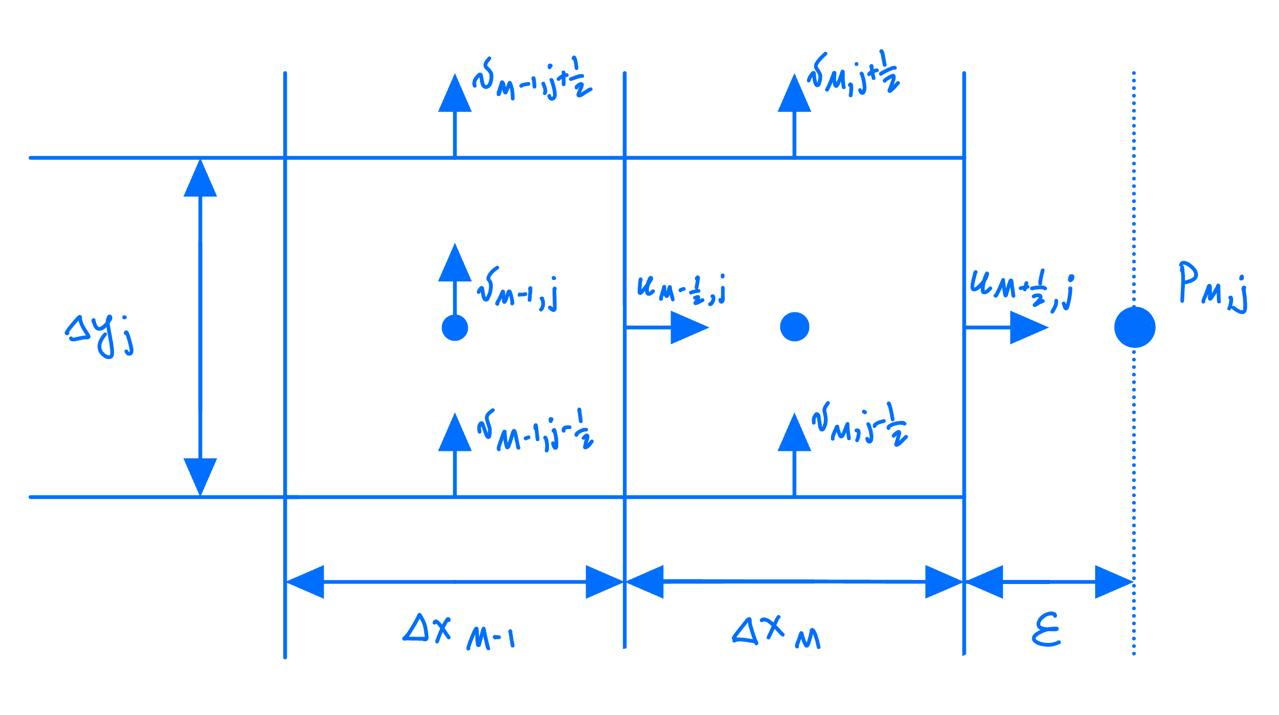
\includegraphics[width=0.45\paperwidth]{pressure-bc}
  }
  \caption{Pressure boundary condition at the right boundary ($\epsilon\to 0$).}\label{fig:luxx-bottom}
\end{figure}
Due to $\varepsilon\to 0$, position of $P_{M,j}\to u_{M+\frac{1}{2},j}$. Therefore, it is necessary to evaluate velocity magnitude at coordinate $M+\frac{1}{2},j$. Component $u$ is inherently located at this coordinate, however, $v$ component needs to be extrapolated. This is possible since we already computed all necessary velocity values at previous time step $n$. First derivative $\frac{\partial u^n}{\partial x}$ will be approximated using backward difference. Finally, we obtain contribution to pressure boundary condition vector as
\begin{equation}\label[bc]{eqn:dong-pressure-dirichlet-right}
	p^{n+1}_{M,j}=\epsilon \frac{u^n_{M+\frac{1}{2},j}-u^n_{M-\frac{1}{2},j}}{\Delta x_M}-\frac{1}{4}\left|\left({u}_{M+\frac{1}{2},j}^n\right)^2+\left({v}_{M+\frac{1}{2},j}^n\right)^2\right| \left(1-\operatorname{tanh}\frac{u_{M+\frac{1}{2},j}^n}{U_0\delta}\right).
\end{equation}
Similarly, at the top boundary we get
\begin{equation}\label[bc]{eqn:dong-pressure-dirichlet-top}
	p^{n+1}_{i,N}=\epsilon \frac{v^n_{i,N+\frac{1}{2}}-v^n_{i,N-\frac{1}{2}}}{\Delta x_M}-\frac{1}{4}\left|\left({u}_{i,N+\frac{1}{2}}^n\right)^2+\left({v}_{i,N+\frac{1}{2}}^n\right)^2\right| \left(1-\operatorname{tanh}\frac{v_{i,N+\frac{1}{2}}^n}{U_0\delta}\right).
\end{equation}




\subsection{Laplacian for top and right boundaries}
In \cref{sec:laplacian} we computed discrete Laplacian operator for inner part, wall and inlet. Here we will approximate this operator using artificial boundary conditions. We will first simplify \cref{eqn:dong-velocity-neumann} algebraically. This removes unnecessary numerical calculations involving $p^{n+1}$ term. Taking \cref{eqn:dong-pressure-dirichlet} and plugging it into \cref{eqn:dong-velocity-neumann} leads to
\begin{equation}
\boldsymbol{\hat{n}}\cdot \nabla \boldsymbol{v}^{n+1}=\frac{1}{\epsilon}\left[\left( \epsilon \boldsymbol{\hat{n}} \cdot \nabla \boldsymbol{v}^n \cdot \boldsymbol{\hat{n}}-\frac{1}{2}\left|\boldsymbol{v}^n\right|^2 S_0\left(\boldsymbol{\hat{n}} \cdot \boldsymbol{v}^n\right)\right) 
	\boldsymbol{\hat{n}}+\frac{1}{2}\left|\boldsymbol{v}^n\right|^2 S_0\left(\boldsymbol{\hat{n}} \cdot \boldsymbol{v}^n\right) \boldsymbol{\hat{n}}-\epsilon\left(\nabla \cdot \boldsymbol{v}^n\right) \boldsymbol{\hat{n}}\right], \quad \text { on } \partial \Omega_0,
\end{equation}
which after simplification reads as
\begin{equation}\label[bc]{eqn:dong-velocity-neumann-simplified}
\boldsymbol{\hat{n}}\cdot \nabla \boldsymbol{v}^{n+1}
=	
		\left( 
			\boldsymbol{\hat{n}} \cdot \nabla \boldsymbol{v}^n \cdot \boldsymbol{\hat{n}}
		\right) \boldsymbol{\hat{n}}
		-\left(\nabla \cdot \boldsymbol{v}^n\right) \boldsymbol{\hat{n}}, \quad \text { on } \partial \Omega_0.
\end{equation}
Now we can directly use \cref{eqn:dong-velocity-neumann-simplified} to compute the remaining Laplacian components.

\textbf{Right boundary}.
At $x=1$ we have $\boldsymbol{\hat{n}}=(1,0)$, this reduces \cref{eqn:dong-velocity-neumann-simplified} to
\begin{equation}\label[bc]{eqn:dong-velocity-neumann-right}
\begin{pmatrix}{}
	\frac{\partial{u}}{\partial x}\\
	\frac{\partial{v}}{\partial x}
\end{pmatrix}^{n+1}
=	
\begin{pmatrix}
	 -\frac{\partial v}{\partial y}\\
	0
\end{pmatrix}^n,
\end{equation}
which in discrete form can be written as 
\begin{equation}
	\frac{u_{M+\frac{3}{2},j}^{n+1}-u_{M+\frac{1}{2},j}^{n+1}}{\Delta x_{M+1}}=-\frac{v^n_{M+1,j+\frac{1}{2}}-v^n_{M+1,j-\frac{1}{2}}}{\Delta y_j}.
\end{equation}
Expressing the outer term leads to
\begin{equation}\label{eqn:u-ghost}
	u^{n+1}_{M+\frac{3}{2},j}=-\frac{v^n_{M+1,j+\frac{1}{2}}-v^n_{M+1,j-\frac{1}{2}}}{\Delta y_j}\Delta x_{M+1}+u^{n+1}_{M+\frac{1}{2},j}.
\end{equation}

\begin{figure}[H] % here, bottom, top
  \centering{
  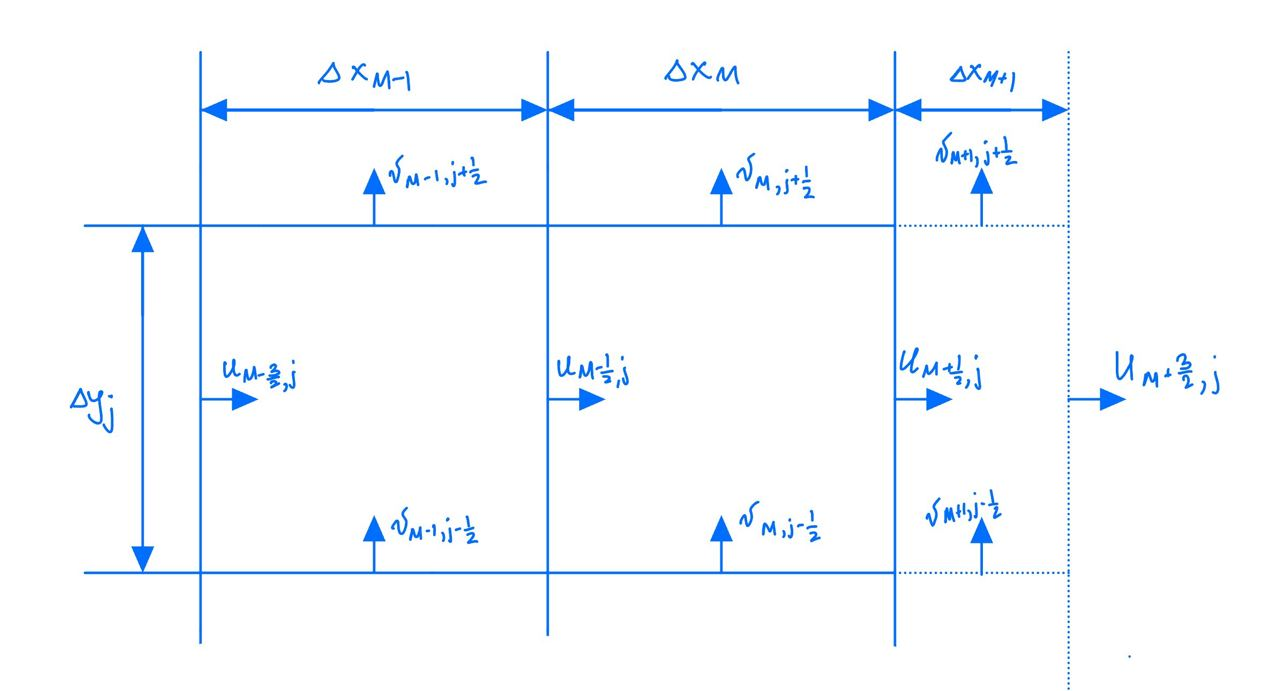
\includegraphics[width=0.45\paperwidth]{luxx-lvxx-right}
  }
  \caption{Laplacian at the right boundary.}\label{fig:luxx-bottom}
\end{figure}

Let us write the second derivative of $u$ w.r.t. $x$ using inner part \cref{eqn:laplacian-discretization-non-uniform-dx} at $M+\frac{1}{2},j$ coordinate 
\begin{equation}
	\left.\frac{\partial^2 u}{\partial x^2}\right|^{n+1}_{M+\frac{1}{2},j}=
		u^{n+1}_{M-\frac{1}{2},j}\frac{1}{\frac{\Delta x_M+\Delta x_{M+1}}{2} \Delta x_M}
		+u^{n+1}_{M+\frac{1}{2},j}\frac{-2}{\Delta x_M \Delta x_{M+1}}
		+u^{n+1}_{M+\frac{3}{2},j}\frac{1}{\Delta x_{M+1}\frac{\Delta x_M+\Delta x_{M+1}}{2}},
\end{equation}
denoting $h_w=x_M,h_e=x_{M+1},h_c=\frac{\Delta x_M+\Delta x_{M+1}}{2}$ gives
\begin{equation}
	\left.\frac{\partial^2 u}{\partial x^2}\right|^{n+1}_{M+\frac{1}{2},j}=
		u^{n+1}_{M-\frac{1}{2},j}\frac{1}{h_w h_c}
		+u^{n+1}_{M+\frac{1}{2},j}\frac{-2}{h_e h_w}
		+u^{n+1}_{M+\frac{3}{2},j}\frac{1}{h_e h_c}.
\end{equation}
We can substitute value of $u^{n+1}_{M+\frac{3}{2},j}$ from \cref{eqn:u-ghost} into the above expression
\begin{align}
	\left.\frac{\partial^2 u}{\partial x^2}\right|^{n+1}_{M+\frac{1}{2},j}&=
		u^{n+1}_{M-\frac{1}{2},j}\frac{1}{h_w h_c}
		+u^{n+1}_{M+\frac{1}{2},j}\frac{-2}{h_e h_w}
		+\left( -\frac{v^n_{M+1,j+\frac{1}{2}}-v^n_{M+1,j-\frac{1}{2}}}{\Delta y_j}\Delta h_e+u^{n+1}_{M+\frac{1}{2},j}\right)\frac{1}{h_e h_c}\\
		&=u^{n+1}_{M-\frac{1}{2},j}\frac{1}{h_c h_w}
		-\frac{\frac{1}{\Delta y}\left( v^n_{M+1,j+\frac{1}{2}}-v^n_{M+1,j-\frac{1}{2}} \right)}{h_c}
		+u^{n+1}_{M+\frac{1}{2},j}\frac{h_w-2h_c}{h_c h_e h_w}.
\end{align}
Simplification using $h_e=h_w-2h_c$ leads to 
\begin{equation}\label{eqn:luxx-right-penulti}
	\left.\frac{\partial^2 u}{\partial x^2}\right|^{n+1}_{M+\frac{1}{2},j}=
	u^{n+1}_{M-\frac{1}{2},j}\frac{1}{h_c h_w}
	-\frac{\frac{1}{\Delta y}\left( v^n_{M+1,j+\frac{1}{2}}-v^n_{M+1,j-\frac{1}{2}} \right)}{h_c}
	+u^{n+1}_{M+\frac{1}{2},j}\frac{1}{h_c h_w}.
\end{equation}
\cref{eqn:luxx-right-penulti} is independent on $h_e$, therefore, we can set $h_e\to 0$, such process will also shift $v$ components locations from $v_{M+1,j+\frac{1}{2}},v_{M+1,j-\frac{1}{2}}$ to $v_{M+\frac{1}{2},j+\frac{1}{2}},v_{M+\frac{1}{2},j-\frac{1}{2}}$. Finally, we can express $\hat{L}^u_{xx}$ together with the corresponding boundary contribution $\hat{L}^u_{\hat{bc}_1}$.

\begin{equation}
	\left.\hat{L}^u_{xx}\right|_{M+\frac{1}{2},j}+\left.\hat{L}^u_{\hat{bc}_1}\right|_{M+\frac{1}{2},j}
	\iff 
	\left[u^{n+1}_{M-\frac{1}{2},j}\frac{1}{h_c h_w}
	+u^{n+1}_{M+\frac{1}{2},j}\frac{1}{h_c h_w}\right]
	-\left[\frac{\frac{1}{\Delta y}\left( v^n_{M+1,j+\frac{1}{2}}-v^n_{M+1,j-\frac{1}{2}} \right)}{h_c}\right].
\end{equation}


Let us rewrite \cref{eqn:laplacian-discretization-non-uniform-dx} for $v$ component at $M,j-\frac{1}{2}$ as
\begin{equation}\label{eqn:laplacian-discretization-v-right-deltax}
\left.\frac{\partial^2 v}{\partial x^2}\right|^{n+1}_{M,j-\frac{1}{2}}=
\frac{
	v^{n+1}_{M-1,j-\frac{1}{2}}\left(\frac{\Delta x_M + \Delta x_{M+1}}{2}\right)
	+v^{n+1}_{M,j-\frac{1}{2}}\left(-\frac{\Delta x_M + \Delta x_{M+1}}{2}-\frac{\Delta x_{M-1} + \Delta x_{M}}{2}\right)
	+v^{n+1}_{M+1,j-\frac{1}{2}}\left(\frac{\Delta x_{M-1} + \Delta x_M}{2}\right)
}
{\frac{\Delta x_{M} + \Delta x_{M+1}}{2} \frac{\frac{\Delta x_M + \Delta x_{M+1}}{2}+\frac{\Delta x_{M-1} + \Delta x_{M}}{2}}{2} \frac{\Delta x_{M-1} + \Delta x_M}{2}}.
\end{equation}
Since the second line in \cref{eqn:dong-velocity-neumann-right} reads as $\frac{\partial v}{\partial x}^{n+1}=0$ we use second order central difference at the boundary index $M+\frac{1}{2},j-\frac{1}{2}$
\begin{equation}
	\left.\frac{\partial v}{\partial x}\right|^{n+1}_{M+\frac{1}{2},j-\frac{1}{2}}=\frac{v^{n+1}_{M+1,j-\frac{1}{2}}-v^{n+1}_{M,j-\frac{1}{2}}}{\frac{\Delta x_{M} + \Delta x_{M+1}}{2}}
\end{equation}
to express 
\begin{equation}\label{eqn:v-right-ghost}
	v^{n+1}_{M+1,j-\frac{1}{2}}=v^{n+1}_{M,j-\frac{1}{2}}.
\end{equation}
Plugging \cref{eqn:v-right-ghost} into \cref{eqn:laplacian-discretization-v-right-deltax} we obtain expression
\begin{equation}\label{eqn:laplacian-v-right-delta}
	\left.\hat{L}^v_{xx}\right|_{M+\frac{1}{2},j-\frac{1}{2}}+\left.\hat{L}^v_{\hat{bc}_1}\right|_{M+\frac{1}{2},j-\frac{1}{2}}
	\iff 
	\frac{
	v^{n+1}_{M-1,j-\frac{1}{2}}\left(\frac{\Delta x_M + \Delta x_{M+1}}{2}\right)
	+v^{n+1}_{M,j-\frac{1}{2}}\left(-\frac{\Delta x_M + \Delta x_{M+1}}{2}\right)
}
{\frac{\Delta x_{M} + \Delta x_{M+1}}{2} \frac{\frac{\Delta x_M + \Delta x_{M+1}}{2}+\frac{\Delta x_{M-1} + \Delta x_{M}}{2}}{2} \frac{\Delta x_{M-1} + \Delta x_M}{2}}.
\end{equation}
The above \cref{eqn:laplacian-v-right-delta} in terms of $h_e=\frac{\Delta x_{M} + \Delta x_{M+1}}{2},h_w=\frac{\Delta x_{M-1} + \Delta x_M}{2},h_c=\frac{\frac{\Delta x_M + \Delta x_{M+1}}{2}+\frac{\Delta x_{M-1} + \Delta x_{M}}{2}}{2}$ is written as
\begin{equation}\label{eqn:laplacian-v-right}
	\left.\hat{L}^v_{xx}\right|_{M+\frac{1}{2},j-\frac{1}{2}}+\left.\hat{L}^v_{\hat{bc}_1}\right|_{M+\frac{1}{2},j-\frac{1}{2}}
	\iff 
	\left[\frac{
	v^{n+1}_{M-1,j-\frac{1}{2}}\left(h_e\right)
	+v^{n+1}_{M,j-\frac{1}{2}}\left(-h_w\right)
}
{ h_w h_c h_e }\right]+\left[0\right].
\end{equation}



\textbf{Top boundary}.



Similarly to \cref{eqn:dong-velocity-neumann-right}, we get 
\begin{equation}\label[bc]{eqn:dong-velocity-neumann-top}
\begin{pmatrix}{}
	\frac{\partial{u}}{\partial x}\\
	\frac{\partial{v}}{\partial x}
\end{pmatrix}^{n+1}
=	
\begin{pmatrix}
	0\\
	 -\frac{\partial u}{\partial x}
\end{pmatrix}^n
\end{equation} 
at top, where $x$ changes to $y$, $u$ changes to $v$ and the rest is verbatim to discretization of corresponding operator at the right boundary that we discussed earlier.






\pagebreak
\section{Normalization}\label{sec:normalization}

The most effective methods for solving systems of linear equations often work optimally with symmetric matrices, making symmetry a desirable property. In order to achieve a symmetric system, we introduce two matrices - the diagonal scaling matrix $\hat{M}$ and the diagonal flux matrix $R$. These matrices are defined as
\begin{align*}
R &\equiv\left[\begin{array}{cc}
\Delta y_j & 0 \\
0 & \Delta x_i
\end{array}\right], \\
\quad \hat{M} & \equiv\left[\begin{array}{cc}
\frac{1}{2}\left(\Delta x_i+\Delta x_{i-1}\right) & 0 \\
0 & \frac{1}{2}\left(\Delta y_j+\Delta y_{j-1}\right)
\end{array}\right].
\end{align*}
 % and $\hat{D}R^{-1}=-(\hat{M}\hat{G})^T$. I THINK THIS WRONG BUT WRITTEN IN TAIRA DISSERTATION ON PAGE 101.

%The only matrix which can be asymmetric in~\cref{eqn:NSE-dsm-bl-system-schemes} is a Laplacian if the grid is non-uniform. In order to get a symmetric diffusion matrix we need to move to the new variables. 
Define matrices 
\begin{equation*}
\begin{aligned}
	\Delta y_j&=\text{diag}([\underbrace{\Delta y_1; \Delta y_1; \dotsc;\Delta y_1}_{M-1\text{ times}}; \underbrace{\Delta y_2; \Delta y_2; \dotsc;\Delta y_2}_{M-1\text{ times}};\dotsc;\underbrace{\Delta y_N; \Delta y_N; \dotsc;\Delta y_N}_{M-1\text{ times}}]),\\
	\Delta x_i&=\text{diag}([\underbrace{\Delta x_1; \Delta x_2;\dotsc\Delta x_M;\Delta x_1; \Delta x_2;\dotsc\Delta x_M; \dotsc;\Delta x_1; \Delta x_2;\dotsc;\Delta x_M}_{N-1\text{ blocks of } 1,\dotsc,M}]),
\end{aligned}
\end{equation*}
which are then combined into
\begin{equation*}
R =\left[\begin{array}{cc}
\Delta y_j & 0 \\
0 & \Delta x_i
\end{array}\right].
\end{equation*}

By moving to new variable ${q} = R\boldsymbol{v}$, we use matrix $R$, which inverse $R^{-1}$ performs half of the symmetrization process for $\hat{L}$. 
Here, $R$ is a diagonal matrix of size $(M-1)N\times M(N-1)$.  Using the $R$ matrix we can express mass flux $q^{n+1}=R\boldsymbol{v}^{n+1}\implies \boldsymbol{v}^{n+1}=R^{-1}q^{n+1}$. It is required that the difference matrices cancel out $\frac{x_{i+1}-x_{i-1}}{2}$ central term in diffusion discretization to make Laplacian partially symmetric. Define the elements of diagonal mass matrix as
\begin{equation*}
{\Delta x_i+\Delta x_{i-1}} = \text{diag}[\underbrace{\Delta x_2+\Delta x_1; \Delta x_3+\Delta x_2; \dotsc ;\Delta x_{M}+\Delta x_{M-1}; ...;\Delta x_2+\Delta x_1; \Delta x_3+\Delta x_2; \dotsc \Delta x_{M}+\Delta x_{M}}_{N\text{ times for each block of } \Delta x_2+\Delta x_1\text{ to }\Delta x_{M}+\Delta x_{M-1}}]
\end{equation*}
and
\begin{equation*}
{\Delta y_j+\Delta y_{j-1}} = \text{diag}[\underbrace{\Delta y_2+\Delta y_1;  \dotsc \Delta y_2+\Delta y_1;}_{M\text{ times}} \underbrace{\Delta y_3+\Delta y_2; \dotsc \Delta y_3+\Delta y_2;}_{M\text{ times}} \underbrace{\Delta y_N+\Delta y_{N-1}\dotsc \Delta y_N+\Delta y_{N-1}}_{M\text{ times}}],	
\end{equation*}
which are then combined into
\begin{equation*}
\hat{M} =\left[\begin{array}{cc}
\frac{1}{2}\left(\Delta x_i+\Delta x_{i-1}\right) & 0 \\
0 & \frac{1}{2}\left(\Delta y_j+\Delta y_{j-1}\right)
\end{array}\right].
\end{equation*}
This matrix both removes the $M^{-1}$ in $\hat{G}=\hat{M}^{-1}G$ if left multiplied and completes the symmetrization process of $\hat{L}$.

Identity ${q}=R\boldsymbol{v}$ implies $\boldsymbol{v}=R^{-1}{q}$, therefore, Laplacian matrix multiplied by the velocity vector becomes
$$\hat{L}\boldsymbol{v}= \hat{L}R^{-1}{q}.$$ 
Premultiplying by $\hat M$ we obtain
$$\hat M\hat{L}R^{-1}{q},$$ 
where $\hat M L R^{-1}$ is symmetric by construction, hence, $\hat M\hat{A}R^{-1}=\hat M (\frac{1}{\Delta t}\mathbf{I}-\frac{1}{2}L) R^{-1}$ is also symmetric.  

Using the above transformations we can modify \cref{eqn:NSE-dsm-bl-system-nonint}
%\begin{equation*}
%\left[\begin{array}{ccc}
%\hat{A} & \hat{G} \\
%\hat{D} & 0 
%\end{array}\right]\left(\begin{array}{c}
%\boldsymbol{v}^{n+1} \\
%p
%\end{array}\right)=\left(\begin{array}{c}
%\hat{r}^n \\
%0 
%\end{array}\right)+\left(\begin{array}{c}
%\widehat{bc}_1 \\
%\widehat{bc}_2 
%\end{array}\right)
%\end{equation*}
into 
\begin{equation*}
\left[\begin{array}{cc}
\hat{M}\hat{A}R^{-1} & \hat{M}\hat{G} \\
\hat{D}R^{-1} & 0
\end{array}\right]\left(\begin{array}{c}
q^{n+1} \\
p^{n+1}
\end{array}\right)=\left(\begin{array}{c}
\hat{M}\hat{r}^n \\
0
\end{array}\right)+\left(\begin{array}{c}
\hat{M}\widehat{b c}_1 \\
\widehat{b c}_2
\end{array}\right),
\end{equation*}
which can be rewritten as 
\begin{equation}\label[system]{eqn:nse-normalized}
\boxed{\left[\begin{array}{cc}
A & G \\
D & 0
\end{array}\right]\left(\begin{array}{c}
q^{n+1} \\
p^{n+1}
\end{array}\right)=\left(\begin{array}{c}
r^n \\
0
\end{array}\right)+\left(\begin{array}{c}
{b c}_1 \\
{b c}_2
\end{array}\right),}
\end{equation}
where $A=\hat{M}\hat{A}R^{-1}=\frac{1}{\Delta t}\hat{M}R^{-1}-\frac{1}{2}\hat{M}\hat{L}R^{-1}$ is symmetric and $\hat{G}=\hat{M}^{-1}G$ according to \cref{eqn:gradient-matrix}. It is also possible to transform the divergence operator $\hat{D}$ with non-integer coefficients into $D$ with integer coefficients in continuity part of \cref{eqn:nse-normalized} using  \cref{eqn:divergence-matrix}. Multiplying both sides of continuity equation by $\Delta _{xy}$ matrix from \cref{eqn:delta-xy} leads to 
\begin{align*}
	\hat{D}\boldsymbol{v}^{n+1}&= \hat{bc}_2,\notag\\
	\left(\Delta_{xy} \right)\hat{D}\boldsymbol{v}^{n+1}&=\left ( \Delta_{xy}\right ) \hat{bc}_2,\notag\\
	\left(\Delta_{xy}\right)\frac{1}{\Delta _{xy}}{D}R\boldsymbol{v}^{n+1}&=\left ( \Delta_{xy}\right ) \hat{bc}_2,\notag\\
	\left(\Delta_{xy}\right)\frac{1}{\Delta_{xy}}{D}q^{n+1}&=\left ( \Delta_{xy}\right ) \hat{bc}_2,\notag\\
	D{q}^{n+1}&=bc_2.
\end{align*}



\pagebreak
\section{Resulting algorithm}\label{sec:algorithm}
Let us consider the solution to discretized \cref{eqn:nse-normalized}
\begin{equation*}
	q^{n+1}=q^{n+1}_p+q^{n+1}_h,
\end{equation*}
where $q^{n+1}_h$ is a solution of homogeneous continuity equation 
\begin{equation}\label{eqn:discrete-homogeneous-continuity}
	Dq^{n+1}_h=0,
\end{equation}
and $q^{n+1}_p$ is a particular solution to its non-homogeneous counterpart
\begin{equation}\label{eqn:discrete-non-homogeneous-continuity}
	Dq^{n+1}_p=bc_2.
\end{equation}
Since we eliminated any explicit boundary condition treatment of the incompressibility constraint and there is no change in density we obtain $bc_2=0$. Hence, it is not required to solve inhomogeneous \cref{eqn:discrete-non-homogeneous-continuity}.
%%%%%%%%%%%%%%
% REMOVE SOURCE TERM BELOW? S_1
%%%%%%%%%%%%%%

We assume that momentum equation from \cref{eqn:nse-normalized} is modified to streamfunction \cref{eqn:biharmonic-streamfunction}, where biharmonic operator satisfies homogeneous \cref{eqn:discrete-homogeneous-continuity} as in Colonius-Taira \cite{Colonius:2008}. 

Taking into account continuous operator identities in \cref{sec:prelude-algorithm}, the resulting algorithm for discrete Navier-Stokes \cref{eqn:nse-normalized} can be described as follows:
\begin{enumerate}
	\item Construct $\operatorname{curl}$ matrix $C$, such that $DC=0$ and $q_h=C\psi$.\label[step]{step:1}
	\item Rewrite $q^{n+1}=q^{n+1}_h$.\label[step]{step:2}
	\item Precompute $bc_1^n$ and $r^n$. \label[step]{step:3}
	\item Eliminate pressure terms in the momentum equation.\label[step]{step:4}
		\begin{align}
			Aq^{n+1}&=-Gp^{n+1}+r^n+bc_1^n,\notag\\
			A(q^{n+1}_h)&=D^Tp^{n+1}+r^n+bc_1^n, &\text{ premultiply by $C^T$,} \notag\\
			C^TAq^{n+1}_h&=C^T(r^n+bc_1^n), &\text{ use $q^{n+1}_h=C\psi^{n+1}$,}\notag\\
			C^TAC\psi^{n+1}&=C^T(r^n+bc_1^n)\label[system]{eqn:resulting-system}.
		\end{align}
		
	\item Solve the resulting \cref{eqn:resulting-system} for $\psi^{n+1}$. This \cref{eqn:resulting-system} is equivalent to biharmonic \cref{eqn:biharmonic-streamfunction}. \label[step]{step:5}
	\item Obtain $q_h^{n+1}=C\psi^{n+1}$.\label[step]{step:6}
	\item Compute $q^{n+1}=q^{n+1}_h$ and convert it to velocity vector field $\boldsymbol{v}^{n+1}=R^{-1}q^{n+1}$.\label[step]{step:7}
	\item Transition to next time instance by repeating \cref{step:3,step:4,step:5,step:6,step:7}.
\end{enumerate}




%\subsection{A particular solution to the discrete continuity equation}\label{sec:particular-solution}
%\pagebreak
%\section{Particular solution using Lagrange multipliers}\label{sec:particular-solution}
%It is possible to find one particular solution to the discrete non-homogeneous continuity \cref{eqn:discrete-non-homogeneous-continuity} using the method of Lagrange multipliers as follows
%\begin{equation}\label{eqn:lagrange-multipliers}
%	Dq_p^{n+1}=bc_2,\implies \mathcal{L}(q_p,\lambda)=
%\|q_p\|^2+\lambda^T(bc_2-D q_p).
%\end{equation}
%
%Differentiating w.r.t $q_p$ and finding the minimum (derivative equal to zero) yields to
%\begin{equation}\label{eqn:flux-minimum}
%2 q_p-D^T \lambda=0.
%\end{equation}
%
%We may premultiply by $D$ to obtain
%\begin{equation*}
%2 D q_p-D D^T \lambda=0,
%\end{equation*}
%then the substitution of $bc_2=D q_p$ will lead to
%
%\begin{equation*}
%\begin{aligned}
%2 bc_2&=D D^T \lambda,\\
%\lambda &=2\left(D D^T\right)^{-1} bc_2,
%\end{aligned}
%\end{equation*}
%plugging the above into~\cref{eqn:flux-minimum} results in
%\begin{equation*}
%q_p=D^T\left(D D^T\right)^{-1} bc_2=D^\dagger bc_2,
%\end{equation*}
%where $D^\dagger=D^T\left(D D^T\right)^{-1}$ is called pseudo-inverse. In the method above we minimize the square of the mass flux, which is equivalent to the minimization of kinetic energy. 
 
%%%% REMOVE?$ %%%%%
%\subsubsection{Particular solution using Graph Theory}\label{subsubsec:particular-graph-theory}
%\textbf{TO KEEP OR NOT TO KEEP}
%Another option to find a particular solution to~\eqref{eqn:discrete-non-homogeneous-continuity} was proposed by Hall in~\cite{Hall:1980} and \cite{Hall:1985}. The method uses the spanning tree of graph $\mathcal{N}$ which has nodes and edges corresponding to the cell centres and velocity vectors from our grid. This method is discussed below.
%
%Let us write useful notations:
%\begin{itemize}
%	\item $\mathcal{N}$ - directed planar network (graph). 
%	\item $K$ - a set of nodes (control volume centres). 
%	
%	$N$ - number of nodes. 
%	\item $\Lambda$ - a set of interior $\Lambda^0$ and boundary $\partial \Lambda$ links (face velocities). 
%		
%		$M$ - total number of links.
%		
%		$M^0$ - number of interior links. 
%	\item Pendant node - a node which is an extremity of only one interior link.  
%	\item $\mathcal{T}$ - a spanning tree of directed network $\mathcal{N}$. $\mathcal{T}$ is a connected partial network of $\mathcal{N}$ which has no cycles.
%\end{itemize}
%
%The procedure for finding a particular solution is as follows:
%\begin{enumerate}
%	\item Construct a spanning tree $\mathcal{T}$ of $\mathcal{N}$ with the pressure specified nodes appended.
%	\item Velocities associated with links not in the tree are set to zero.
%	\item Choose a node in $\mathcal{T}$ which is an extremity of a boundary link and call it root. 
%	\item Set the boundary link velocities equal to zero, except the link incident on the root.
%	\item At each pendant node except the root, the continuity equation was reduced to a simple equation relating the velocity only at the internal connection of the tree to that node.  
%	\item Move from the pendant node along the tree towards the root. At each node the continuity equation involves a single unknown velocity.
%	\item Except the juncture nodes, where the chains from one or more pendant nodes connect. Before solving the continuity equation associated with such a juncture node, the velocities on the chains from pendant nodes to the juncture node have to be determined.
%	\item The process is completed after using the continuity equation at the root to determine the final velocity of the boundary link.
%\end{enumerate}

%Let us take our momentum equation and apply the equation~\eqref{eqn:non-homogeneous} to it.
%	\begin{equation}
%	\begin{aligned}
%		Aq + Gp & =bc_1,\text{ premultiply by } C^T,\\
%		C^T A q+0 & =C^T bc_1, \\
%		C^TA(C\psi+q_p)&=C^T bc_1,\\
%		C^TA C\psi&=C^T bc_1 - C^TA q_p,\\
%		C^TA C \psi & = C^T bc_1 - C^TA D_p^\dagger bc_2.
%	\end{aligned}
%	\end{equation}

%Let us apply boundary conditions to matrix $D$, and call it $D_p$. Using the method described above we find one particular solution $q_p$  to the non-homogeneous continuity equation~\eqref{eqn:discrete-continuity}, but with $D_p$, which has the boundary conditions (Dirichlet, Neuman, or mixed) applied. 
%
%\begin{equation}
%	q_p=D_p^\dagger bc_2.
%\end{equation}
%
%Then, the final system of equations to be solved can be constructed using $q=q_h+q_p$ with two choices (\textbf{TO BE DETERMINED}):
%\begin{enumerate}
%	\item First choice is based on the assumption that the momentum equation has the solution of both particular and homogeneous continuity equation.
%	\begin{equation}
%	\begin{aligned}
%		Aq + Gp & =bc_1,\text{ premultiply by } C^T,\\
%		C^T A q+0 & =C^T bc_1, \\
%		C^TA(q_h+q_p)&=C^T bc_1,\\
%		C^TA q_h&=C^T bc_1 - C^TA q_p,\\
%		C^TA C \psi_h & = C^T bc_1 - C^TA D_p^\dagger bc_2.
%	\end{aligned}
%	\end{equation}
%	\item Second choice is based on the assumption that the momentum equation has the solution of homogeneous continuity equation only, which feels making more sense, since in this case $G=-D_h^T$ and will kill pressure term, where $D$ has pure Dirichlet =0 boundary conditions.
%	\begin{equation}
%	\begin{aligned}
%		Aq_h + Gp & =bc_1,\text{ premultiply by } C^T,\\
%		C^T A q_h+0 & =C^T bc_1, \\
%		C^TA(q-q_p)&=C^T bc_1,\\
%		C^TA q&=C^T bc_1 + C^TA q_p,\\
%		C^TA C \psi & = C^T bc_1 + C^TA D_p^\dagger bc_2.
%	\end{aligned}
%	\end{equation}
%\end{enumerate}

%\section{Other interesting methods for solving Naver Stokes (may include algorithms from articles \cite{Brown:2001, Dukowicz:1992, Kim:1985, Perot:1993})}
%
%Citing Colonius~\cite{Colonius:2008} The second type of error associated with vorticity advecting or diffusing through the boundary is typically handled by posing outflow boundary conditions. For incompressible flow, these are usually called convective boundary conditions, whereas for compressible flow the term non-reflecting boundary condition is often used. Multidomain boundary conditions used on 3 domains: fine, medium, and coarse. 
	
\section{Summary}\label{sec:summary}
	

\pagebreak
\bibliographystyle{plain}
\bibliography{Zotero.bib}


\pagebreak
\appendix
%\section{Appendix}
\section{Treating boundary conditions implicitly and maintaining the symmetric property of system}
Consider the following discrete Poisson equation 
\begin{equation}
\left[
\begin{array}{ccc|c|cccc}
-4 & 1 & 1 & 0 & 0 & 0 & 0 & 0 \\
1 & -4 & 0 & 1 & 0 & 0 & 0 & 0 \\
1 & 0 & -4 & 1 & 0 & 0 & 0 & 0 \\
\hline
0 & 0 & 0 & 1 & 0 & 0 & 0 & 0 \\
\hline
0 & 0 & 0 & 0 & -4 & 1 & 1 & 0 \\
0 & 0 & 0 & 0 & 1 & -4 & 0 & 1 \\
0 & 0 & 0 & 0 & 1 & 0 & -4 & 1 \\
0 & 0 & 0 & -1 & 0 & 1 & 1 & -4
\end{array}
\right]
\left[
\begin{array}{c}
u_1\\
u_2\\
u_3\\
u_4\\
u_5\\
u_6\\
u_7\\
u_8
\end{array}
\right]
=\left[
\begin{array}{c}
r_1\\
r_2\\
r_3\\
r_4\\
r_5\\
r_6\\
r_7\\
r_8
\end{array}
\right].
\end{equation}
Row 4 is treating boundary condition of the corresponding unknown $u_4$ implicitly. Let us multiply the whole row by a very large number $10^{10}$.
\begin{equation}
\left[
\begin{array}{ccc|c|cccc}
-4 & 1 & 1 & 0 & 0 & 0 & 0 & 0 \\
1 & -4 & 0 & 1 & 0 & 0 & 0 & 0 \\
1 & 0 & -4 & 1 & 0 & 0 & 0 & 0 \\
\hline
0 & 0 & 0 & 10^{10} & 0 & 0 & 0 & 0 \\
\hline
0 & 0 & 0 & 0 & -4 & 1 & 1 & 0 \\
0 & 0 & 0 & 0 & 1 & -4 & 0 & 1 \\
0 & 0 & 0 & 0 & 1 & 0 & -4 & 1 \\
0 & 0 & 0 & -1 & 0 & 1 & 1 & -4
\end{array}
\right].
\left[
\begin{array}{c}
u_1\\
u_2\\
u_3\\
u_4\\
u_5\\
u_6\\
u_7\\
u_8
\end{array}
\right]
=\left[
\begin{array}{c}
r_1\\
r_2\\
r_3\\
10^{10}r_4\\
r_5\\
r_6\\
r_7\\
r_8
\end{array}
\right]
\end{equation}
Let us now add or subtract any relatively small constants from different columns of this row. In order to make the matrix symmetric we can modify it to
\begin{equation}
\left[
\begin{array}{ccc|c|cccc}
-4 & 1 & 1 & 0 & 0 & 0 & 0 & 0 \\
1 & -4 & 0 & 1 & 0 & 0 & 0 & 0 \\
1 & 0 & -4 & 1 & 0 & 0 & 0 & 0 \\
\hline
0 & 1 & 1 & 10^{10} & 0 & 0 & 0 & -1 \\
\hline
0 & 0 & 0 & 0 & -4 & 1 & 1 & 0 \\
0 & 0 & 0 & 0 & 1 & -4 & 0 & 1 \\
0 & 0 & 0 & 0 & 1 & 0 & -4 & 1 \\
0 & 0 & 0 & -1 & 0 & 1 & 1 & -4
\end{array}
\right]
\left[
\begin{array}{c}
u_1\\
u_2\\
u_3\\
u_4\\
u_5\\
u_6\\
u_7\\
u_8
\end{array}
\right]
=\left[
\begin{array}{c}
r_1\\
r_2\\
r_3\\
10^{10}r_4\\
r_5\\
r_6\\
r_7\\
r_8
\end{array}
\right].
\end{equation}
Row 4 now becomes
$u_2+u_3+10^{10}u_4-u_8\approx 10^{10} u_4$, since relatively small values of $u_2,u_3,u_8$ can be treated as round-off errors.  

%\subsection{Transient schemes}

\end{document}
